%!TeX program = lualatex

\documentclass[oneside]{academica}
\usepackage{parskip}
\usepackage{enumitem}

\usetikzlibrary{shapes.misc}
\tikzset{cross/.style={cross out, draw, minimum size=4pt, inner sep=0pt, outer sep=0pt}}

\colorlet{fg}{black}
\colorlet{bg}{white}

\newcommand{\diff}[2]{\frac{\partial #1}{\partial #2}}


\overtitle{notes for}
\title{Deep Learning}
\author{Filippo Merlo}
\date{2023-2024}

\begin{document}

\frontmatter

\maketitle

\tableofcontents

\mainmatter

\chapter{Introduction}

\begin{minipage}{0.6\linewidth}
The general definitions for Artificial intelligence are:
  \begin{itemize}
    \item \textbf{Artificial Intelligence} = any technique which enables computers to mimic human behaviors.
    \item \textbf{Machine Learning} = uses statistical methods to improve the machine behavior.
    \item \textbf{Deep Learning} based on neural networks, extracts patterns from raw data to improve artificial intelligence.
  \end{itemize}
\end{minipage}
\hspace{0.02\linewidth}
\begin{minipage}{0.3\linewidth}
  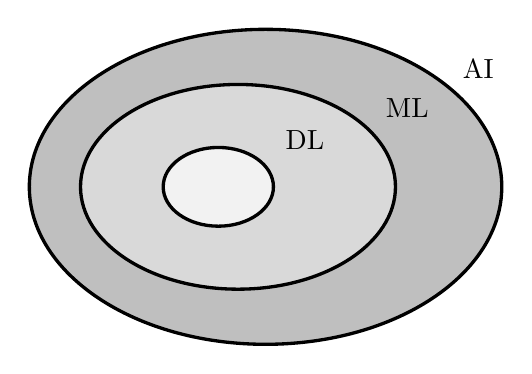
\begin{tikzpicture}
    \draw[very thick, fill=fg!25] (0,0) circle [x radius=3cm, y radius=2cm] (2.7,1.5) node{AI};
    \draw[very thick, fill=fg!15] (-0.35,0) circle [x radius=2cm, y radius=1.3cm] (1.8,1) node{ML};
    \draw[very thick, fill=fg!05] (-0.6,0) circle [x radius=0.7cm, y radius=0.5cm] (0.5,0.6) node{DL};
  \end{tikzpicture}
\end{minipage}
\\\\\\
There are different Machine Learning algorithms:
\begin{itemize}
  \item Supervised learning
  \item Unsupervised learning
  \item Reinforcement learning
  \item Generative Learning
\end{itemize}

\section{Supervised learning}

A system that can solve specific tasks (one at a time).
For an input there will be for sure an output (it doesn't matter if it's correct or wrong).
The AI is trained and its behavior is checked by a real person.
The files/images are labelled manually (e.g. `face' or `no face') by the staff before are given in input to the AI.
All the files with their right classification constitute the dataset; in this way the AI can check its prediction against the right answer present in the dataset.

This type of learning can be furthermore split in two types:
\begin{itemize}
  \item Regression
  \item Classification
\end{itemize}

\newpage

\subsection{Regression}

As we can see in \textit{Figure~\ref{fig:regression mechanism}}, this AI makes numerical predictions.

\begin{figure}[h]
  \begin{center}
    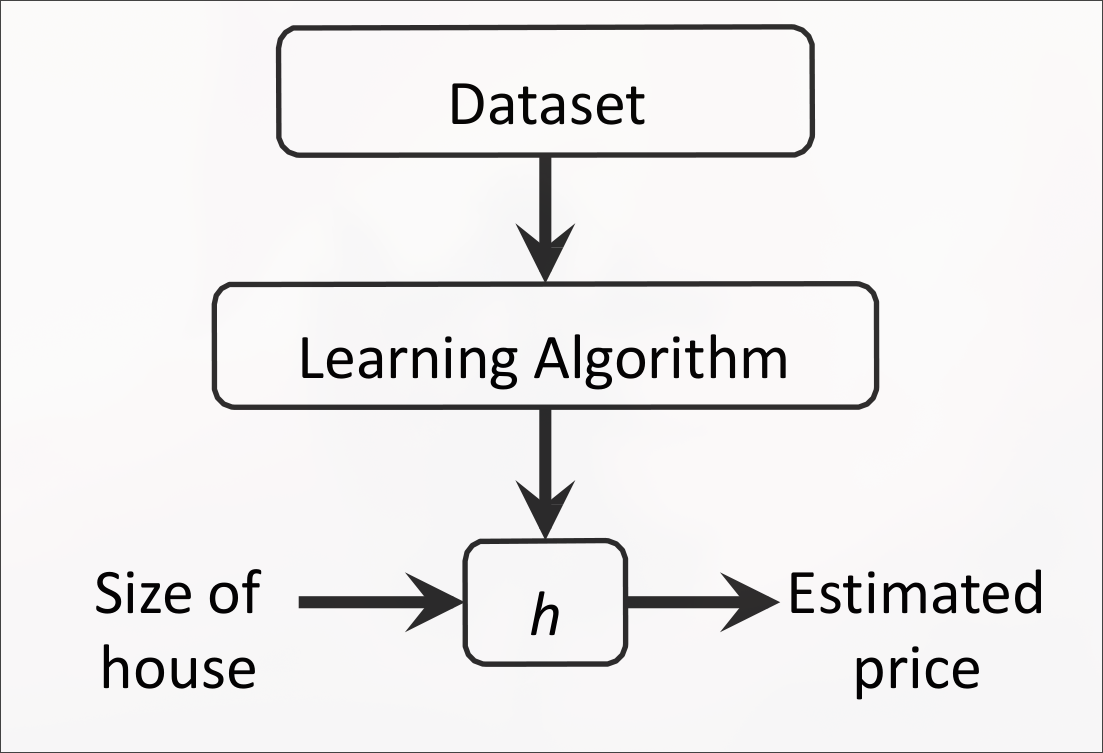
\includegraphics[width=0.4\textwidth]{figures/mechanism}
  \end{center}
  \caption{
    Regression mechanism\\
    $h$ is the decision function
  }\label{fig:regression mechanism}
\end{figure}

It can work over single or multiple features (parameters) of the dataset, like we can see in the two examples below (\textit{Figure~\ref{fig:house_1}} and~\textit{\ref{fig:house_2}}).
In the second case, it's easier for the AI to predict a precise response.

\begin{figure}[h]
  \begin{minipage}{0.48\textwidth}
    \centering
    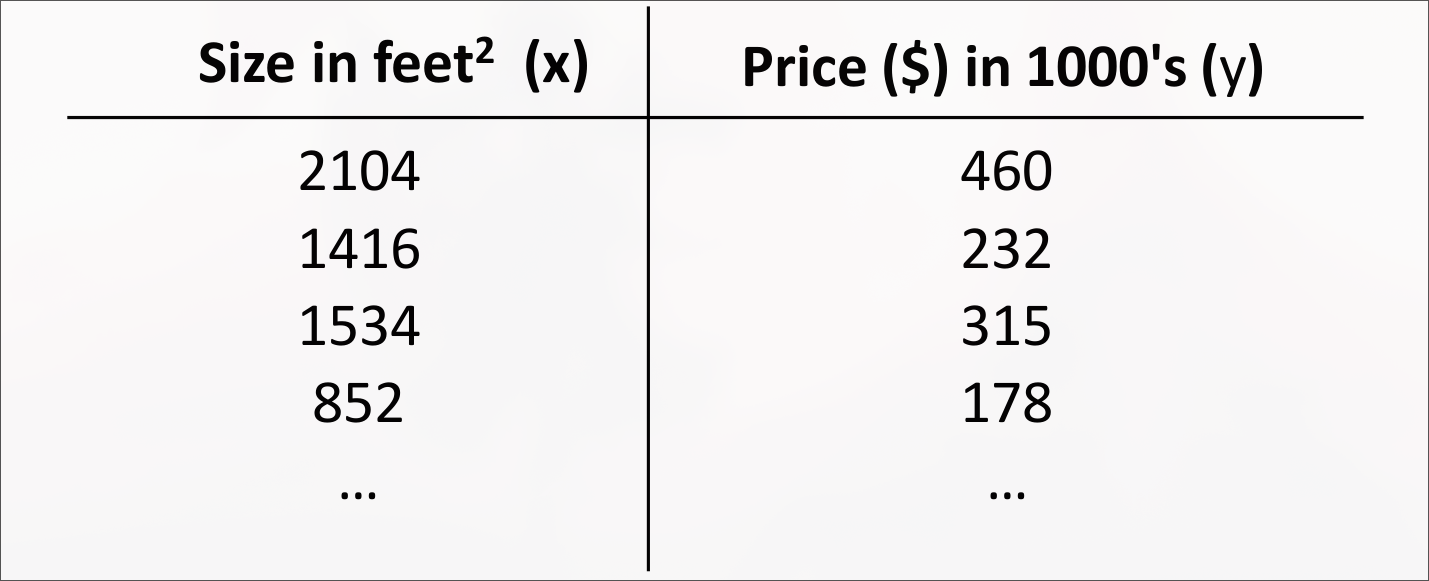
\includegraphics[width=\linewidth, height=3cm]{figures/house_1}
    \caption{Single features}\label{fig:house_1}
  \end{minipage}
  \hfill
  \begin{minipage}{0.48\textwidth}
    \centering
    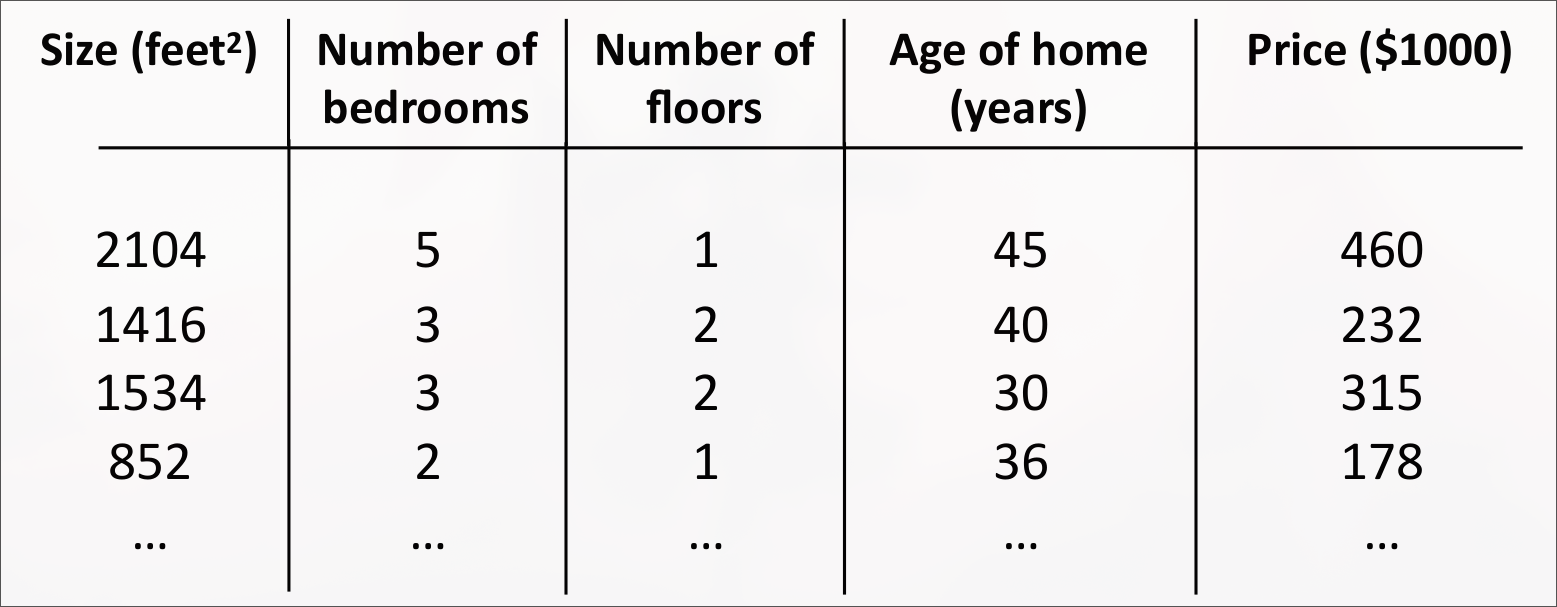
\includegraphics[width=\linewidth, height=3cm]{figures/house_2}
    \caption{Multiple features}\label{fig:house_2}
  \end{minipage}
\end{figure}

\subsection{Classification}

The classification problem is like the regression problem, except that the output domain is restricted and small.
For example, in the \textbf{binary classification problem}, predictions can take on only two values: 0 (``negative class'') or 1 (``positive class'').

A real example of binary classification problem is the following one:

\begin{figure}[h]
  \begin{minipage}{0.5\textwidth}
    \begin{quote}
      \textit{Suppose that we want to classify the tumor size in comparison to the patient age, a possible scenario is the one we can see in \textit{Figure~\ref{fig:tumor classification}} on the side.}
    \end{quote}
  \end{minipage}
  \hspace{50pt}
  \begin{minipage}{0.38\textwidth}
    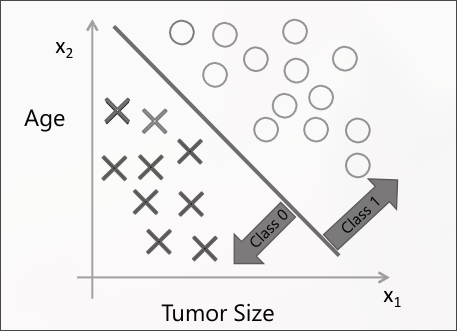
\includegraphics[width=\linewidth]{figures/tumor}
    \caption{Tumor classification}\label{fig:tumor classification}
  \end{minipage}
\end{figure}

The dataset for this type of problem is a set of tuples $(feature_1, feature_2)$ and in the example above the tuples were $(age, size)$.

We can train our AI to decide in which group a person will belong given its dataset.
The AI is also responsible for deciding which is the most reliable and precise grouping (in our example above, the grouping function was the separating line).

\section{Unsupervised learning}

The main difference against the supervised type of learning, is that each result isn't labelled, thus we don't have correct or wrong predictions.
The AI's task, in this type of learning, is to find a grouping of the input data. A \textbf{cluster} is a subset of the input data, which has been grouped because the AI found a similitude between them.

\begin{figure}[h]
  \begin{center}
    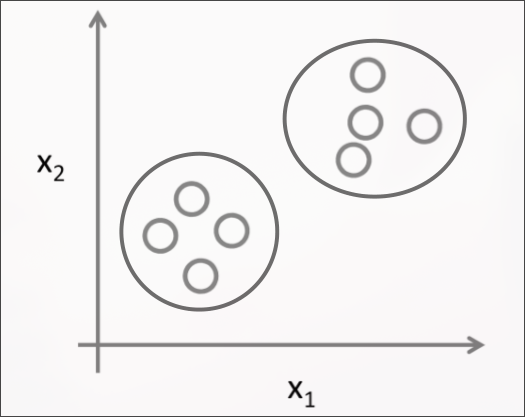
\includegraphics[width=0.35\textwidth]{figures/market_segmentation}
  \end{center}
  \caption{Market segmentation}\label{fig:market segmentation}
\end{figure}

The example in \textit{Figure~\ref{fig:market segmentation}} above, is a market segmentation aimed to improve the selling quantities, based on the people buying.

Netflix, for instance, uses unsupervised learning with the movie thumbnails.
It has 3 or 4 images for each film and with time, the AI is able to create as many clusters as the number of images provided and in each one there will be those people that liked more that thumbnail over the others.
In this way, Netflix is able to decide which type of image is the most effective for you, based on your previous decision history, and show you only the type of thumbnail that you like the most, as a cover for its films.

\section{Reinforcement learning}

\vspace{-15pt}
\begin{figure}[h]
  \begin{minipage}{0.4\textwidth}
    Like in robotics, to train machines to grab, transport or move objects (automation).
  \end{minipage}
  \hspace{40pt}
  \begin{minipage}{0.5\textwidth}
    \begin{center}
      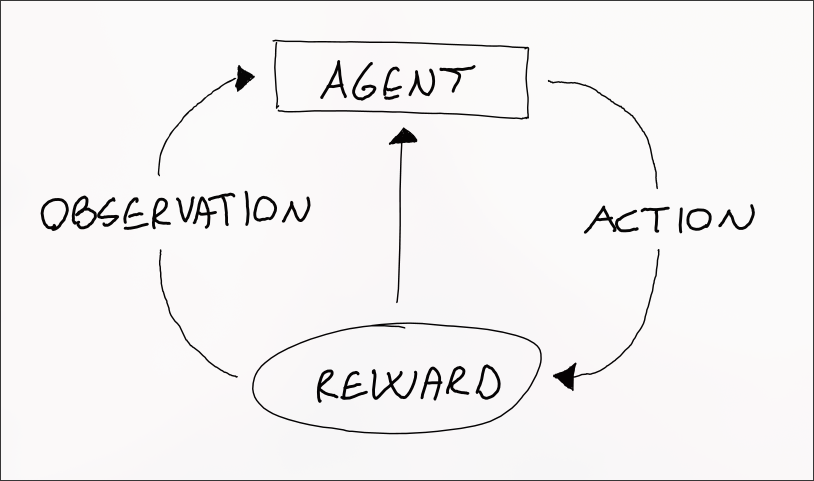
\includegraphics[width=0.8\linewidth]{figures/reinforcement}
    \end{center}
    \caption{Reinforcement learning cycle}\label{fig:reinforcement}
  \end{minipage}
\end{figure}

\chapter{Neural Networks}

\section{Simple example of Neural Network}

A simple neural network example: AND logic port

\begin{figure}[h]
  \begin{minipage}{0.48\textwidth}
    \centering
    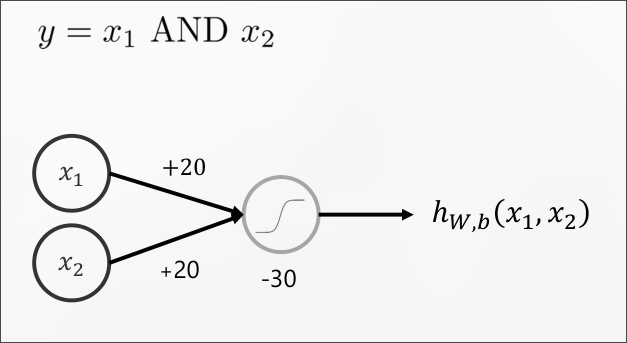
\includegraphics[width=\linewidth]{figures/simple_nn}
    \label{fig:simple_nn}
  \end{minipage}
  \hfill
  \begin{minipage}{0.48\textwidth}
    \vspace{-15pt}
    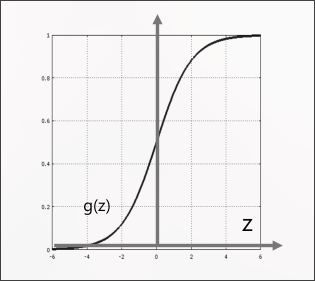
\includegraphics[width=0.8\linewidth, height=4.42cm]{figures/simple_nn_graph}
    \label{fig:simple_nn_graph}
  \end{minipage}
\end{figure}

The equation of the above neural network is

\begin{equation*}
  h_{w,b}(x_1,x_2) = g(wx_1 + wx_2 + b)
\end{equation*}

Where

\begin{itemize}
  \item $\boldsymbol{x}$ is the input
  \item $\boldsymbol{y}$ is the output
  \item $\boldsymbol{h}$ is the activation function with $\boldsymbol{w}$ weight and $\boldsymbol{b}$ bias (error)
  \item $\boldsymbol{g}$ is the sigmoid function
\end{itemize}


\begin{figure}[h]
  \begin{minipage}{0.6\textwidth}
    \textbf{Hidden layers} add complexity without changing the model, weight or bias.
    With an additional intermediate layer, it's possible to add more weights and improve the Neural Network to solve more complex scenarios like in \textit{figure \ref{fig:complex_example}}.

    There will be cases not solvable also with a hidden layer.
    Adding neurons in the hidden layer is another way to increase furthermore the complexity, to make the AI able to solve and classify the data.
  \end{minipage}
  \hfill
  \begin{minipage}{0.35\textwidth}
    \begin{center}
      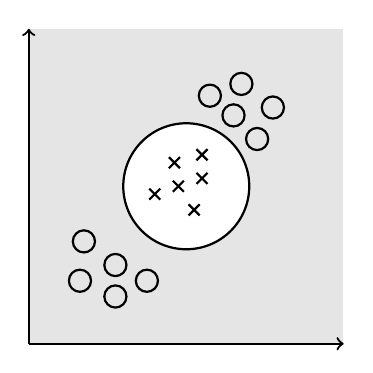
\begin{tikzpicture}
        \filldraw[fill=fg!10, draw=white] (0,0) rectangle (4,4);
        \draw[fill=fg,thick,->] (0,0) -- (4,0);
        \draw[fill=fg,thick,->] (0,0) -- (0,4);

        \draw[thick, fill=white] (2,2) circle (0.8);

        \draw[thick] (1.1,1) circle (4pt);
        \draw[thick] (1.5,0.8) circle (4pt);
        \draw[thick] (1.1,0.6) circle (4pt);
        \draw[thick] (0.7,1.3) circle (4pt);
        \draw[thick] (0.65,0.8) circle (4pt);

        \draw[thick] (3.1,3) circle (4pt);
        \draw[thick] (2.3,3.15) circle (4pt);
        \draw[thick] (2.9,2.6) circle (4pt);
        \draw[thick] (2.7,3.3) circle (4pt);
        \draw[thick] (2.6,2.9) circle (4pt);

        \draw (1.6,1.9) node[thick, cross] {};
        \draw (1.85,2.3) node[thick, cross] {};
        \draw (2.1,1.7) node[thick, cross] {};
        \draw (2.2,2.4) node[thick, cross] {};
        \draw (1.9,2) node[thick, cross] {};
        \draw (2.2,2.1) node[thick, cross] {};
      \end{tikzpicture}
    \end{center}
    \caption{More complex scenario}
    \label{fig:complex_example}
  \end{minipage}
\end{figure}

The output layer has as many nodes as the number of classes.

\newpage

\begin{figure}[h]
  \begin{minipage}{0.48\textwidth}
    \centering
    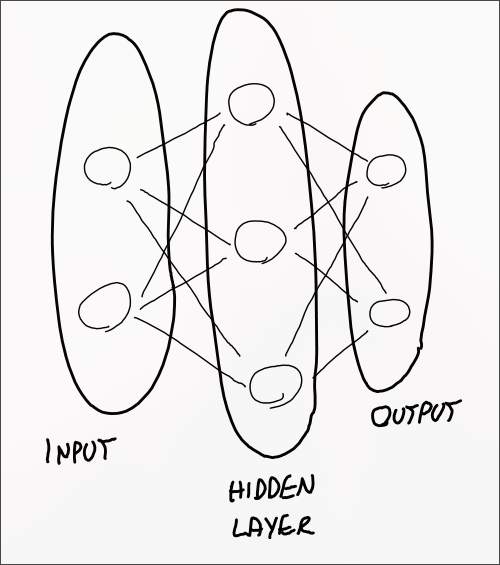
\includegraphics[scale=0.3]{figures/layers}
    \caption{NN's layers}\label{fig:layers}
  \end{minipage}
  \hfill
  \begin{minipage}{0.48\textwidth}
    \begin{center}
      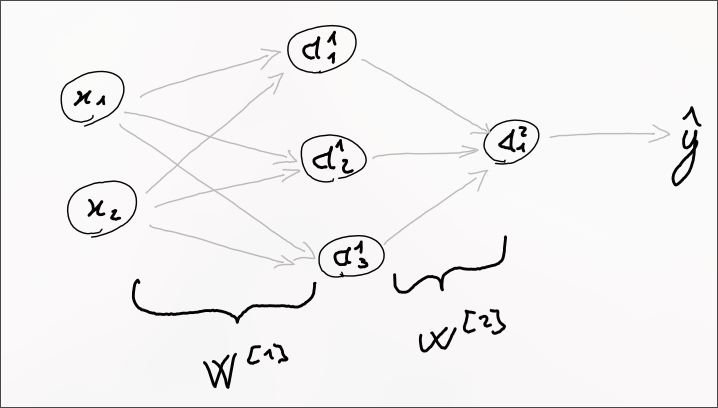
\includegraphics[width=\linewidth]{figures/matrix_of_weights}
    \end{center}
    \caption{Matrixes of weights}\label{fig:matrix_of_weights}
  \end{minipage}
\end{figure}

As we can see in \textit{Figure~\ref{fig:matrix_of_weights}}

\begin{itemize}
  \item $\boldsymbol{\hat{y}}$ is the output
  \item $\boldsymbol{a^{[j]}}$ is the activation vector for layer $j$ and its formula is $a^{[j]} = g^{[j]} \cdot z^{[j]}$, where $z^{[j]}$ is the intermediate function value and its formula is $z^{[j]} = W^{[j]}x + b^{[j]}$.
  \item $\boldsymbol{b^{[j]}}$ is the bias
  \item $\boldsymbol{g^{[j]}}$ is the activation function for layer $j$, which puts the feature's values of $z^{[j]}$ in the prediction space of $a^{[j]}$. An example is the sigmoid function.
  \item $\boldsymbol{W^{[j]}}$ is the matrix of weights, mapping from layer $j-1$ to layer $j$. In the figure $W^{[1]}$  is a matrix $3 \times 2$, while $W^{[2]}$ has size $1 \times 3$.
\end{itemize}

The training of a Neural Network that has been initialized with random weights, is performed by \textbf{backpropagation}.
This technique consists in the repetition of the following steps:
\begin{enumerate}
  \item \textbf{Network activation} (\textit{forward step}): the network is activated and the error of the output layer is computed.
  \item \textbf{Error propagation} (\textit{backward step}): the error that has been computed is used to correct the weight values, starting from the output.
\end{enumerate}

An \textbf{epoch} is a cycle of backpropagation, which corresponds to $n$ back and forth steps (e.g. 10000), until all the dataset is used.
Then, the cycle will be repeated another $m$ number of times.

We are in the training phase, thus we use a dataset where each data is labelled, and we can establish if the prediction of the Neural Network was right or wrong.

\section{Activation function}

The most common activation functions are:
\begin{itemize}
  \item \textbf{Sigmoid}: its formula is $f(x) = \displaystyle \frac{1}{1+e^{-x}}$ which working space is [0,1], thus is used mostly in the final layer before the output, to convert the prediction to that space.
  \item \textbf{Tanh}: $\displaystyle f(x) = \frac{e^x-e^{-x}}{e^x+e^{-x}}$ so its space is in [-1,1].
  \item \textbf{ReLU} (\textit{Rectified Linear Unit}): it's the most used and its definition is
    \begin{equation*}
      y = \left\{
      \begin{aligned}
        & 0, \quad & x \le 0 \\
        & x, \quad & x > 0
      \end{aligned}
      \right.
      \label{eq:ReLU}
    \end{equation*}
  \item \textbf{LeakyReLU}: is born to solve the \textbf{Dying ReLU problem}, where some ReLU ``die'' for all inputs, because the gradient of the function becomes 0 and the network cannot perform backpropagation and learn.
    For this reason $a$ is set to 0.2 instead of 0.
    \begin{equation*}
      y = \left\{
      \begin{aligned}
        ax & , \quad & x \le 0 \\
        x & , \quad & x > 0
      \end{aligned}
      \right.
      \label{eq:LeakyReLU}
    \end{equation*}
\end{itemize}

\begin{minipage}{0.48\textwidth}
  \begin{center}
    \begin{tikzpicture}
      \begin{axis}[
        xmax=10,
        xmin=-10,
        xtick={-10, -5, 0, 5, 10},
        axis x line=middle,
        ymax=1.1,
        ymin=-1.1,
        ytick={-1, -0.5, 0, 0.5, 1},
        axis y line=middle,
        axis line style={-},
        title={\textbf{Sigmoid}}
      ]
        \addplot[
          mark=none,
          samples=100,
          domain=-10:10,
          style={very thick}
        ]
        (x,{1/(1+exp(-x))});
      \end{axis}
    \end{tikzpicture}
  \end{center}
  \vspace{-15pt}
\end{minipage}
\hfill
\begin{minipage}{0.48\textwidth}
  \begin{center}
     \begin{tikzpicture}
      \begin{axis}[
        xmax=10,
        xmin=-10,
        xtick={-10, -5, 0, 5, 10},
        axis x line=middle,
        ymax=1.1,
        ymin=-1.1,
        ytick={-1, -0.5, 0, 0.5, 1},
        axis y line=middle,
        axis line style={-},
        title={\textbf{Tanh}}
      ]
        \addplot[
          mark=none,
          samples=100,
          domain=-10:10,
          style={very thick}
        ]
        (x,{(exp(x)-exp(-x))/(exp(x)+exp(-x))});
      \end{axis}
    \end{tikzpicture}
  \end{center}
  \vspace{-15pt}
\end{minipage}

\vspace{25pt}

\begin{minipage}{0.48\textwidth}
  \begin{center}
    \begin{tikzpicture}
      \begin{axis}[
        xmax=10,
        xmin=-10,
        xtick={-10, -5, 0, 5, 10},
        axis x line=middle,
        ymax=10,
        ymin=-10,
        ytick={-10, -5, 0, 5, 10},
        axis y line=middle,
        axis line style={-},
        title={\textbf{ReLU}}
      ]
        \addplot[
          mark=none,
          samples=100,
          domain=-10:0,
          style={very thick}
        ]
        (x,{0});
        \addplot[
          mark=none,
          samples=100,
          domain=0:10,
          style={very thick}
        ]
        (x,{x});
      \end{axis}
    \end{tikzpicture}
  \end{center}
  \vspace{-15pt}
\end{minipage}
\hfill
\begin{minipage}{0.48\textwidth}
  \begin{center}
    \begin{tikzpicture}
      \begin{axis}[
        xmax=10,
        xmin=-10,
        xtick={-10, -5, 0, 5, 10},
        axis x line=middle,
        ymax=10,
        ymin=-10,
        ytick={-10, -5, 0, 5, 10},
        axis y line=middle,
        axis line style={-},
        title={\textbf{LeakyReLU}}
      ]
        \addplot[
          mark=none,
          samples=100,
          domain=-10:0,
          style={very thick}
        ]
        (x,{0.2*x});
        \addplot[
          mark=none,
          samples=100,
          domain=0:10,
          style={very thick}
        ]
        (x,{x});
      \end{axis}
    \end{tikzpicture}
  \end{center}
  \vspace{-15pt}
\end{minipage}

\vspace{25pt}

Non-linear functions are needed because if before the 1st layer we don't have an activation function, in the next layer we will have a quadratic expression, not solvable through linear functions.

\newpage

\section{Loss function}

It's also called \textbf{cost function} and it measures the ``cost'' of an incorrect prediction in a neural network.
It's represented with $\boldsymbol{\mathcal{L}(\hat{y}, y)}$, where $\boldsymbol{\hat{y}}$ is the predicted value and $\boldsymbol{y}$ is the actual value associated to the given input.

\subsection{Empirical Loss}

We call \textbf{Empirical Loss} the total loss measured over the entire dataset and it's equal to
\begin{equation*}
  J(W,b) = \frac{1}{m} \sum_{i=1}^{m} \mathcal{L}(\hat{y}^{(i)}, y^{(i)})
  \label{eq:empirical loss}
\end{equation*}
and this function is also called \textbf{objective function}.

\subsection{Binary Cross Entropy Loss}

Another useful function is the \textbf{Binary Cross Entropy Loss} and is a loss function used with models that output a probability between 0 and 1.
Its formula is
\begin{equation*}
  J(W,b) = \frac{1}{m} \sum_{i=1}^{m} -[y^{(i)} ln (\hat{y}^{(i)}) +(1 - y^{(i)}) ln (1 - \hat{y}^{(i)})]
  \label{eq: binary cross entropy loss}
\end{equation*}

The cost function is logarithmic.

\begin{figure}[h]
  \begin{center}
    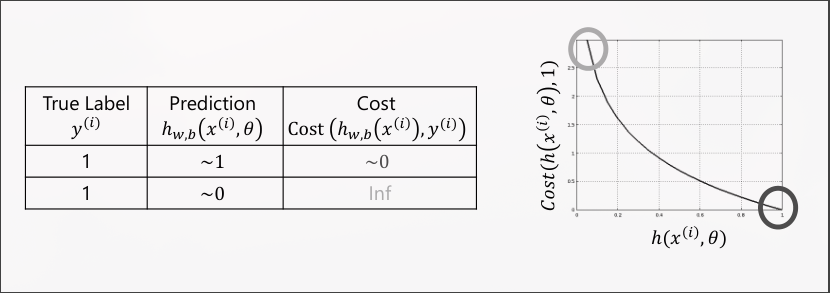
\includegraphics[width=\linewidth]{figures/cost_function}
  \end{center}
  \caption{Cost function diagram}
\end{figure}

\subsection{Mean Squared Error Loss}

It can be used with regression models that output continuous real numbers and its formula is:
\begin{equation*}
  J(W,b) = \frac{1}{m} \sum_{i=1}^{m} (y^{(i)} - \hat{y}^{(i)})^2
  \label{eq:mean squared error loss}
\end{equation*}

\newpage

\section{Training of Neural Networks}

\subsection{Loss Optimization}

It's the problem of finding the network weights and biases that achieve the lowest loss. The formula to compute it is

\begin{equation*}
  J(W,b) = \frac{1}{m} \sum_{i=1}^{m} \mathcal{L}(\hat{y}^{(i)}, y^{(i)})
  \label{eq:loss optimization}
\end{equation*}
\begin{equation*}
  [w^*,b^*] = min_{(W,b)}\ J(W,b)
\end{equation*}

where the domain of the Neural Network are real numbers, $\boldsymbol{\mathcal{L}}$ is the loss function, $\boldsymbol{m}$ is the number of samples and $\boldsymbol{[w^*,b^*]}$ are the best weight and bias of the network.

This technique finds the \textbf{local minimum}, but we're not sure that the found value corresponds also to the global minimum.

\subsection{Gradient Descent}

The gradient descent is an algorithm to minimize a derivable function through linear regression. If the function is not derivable, the algorithm simply will not work.
The algorithm is initialized with random weights and biases $(\theta_0, \dots, \theta_n)$, while, during the execution, these values are changed, in order to reduce the cost $J(\theta_0, \dots, \theta_n)$ and hopefully find a minimum.
The algorithm code is:
\begin{equation*}
  \theta_j \coloneqq \theta_j - \alpha \frac{\partial}{\partial \theta_j} J(\theta_0,\theta_1)
  \label{eq:}
\end{equation*}
to be repeated until convergence. $\boldsymbol{j}$ are the indexes, $\boldsymbol{\alpha}$ is the length/size of the step, $\boldsymbol{J}$ is the cost function and $\boldsymbol{\partial}$ is the partial derivative.

\begin{note}
  The gradient of a function represents how small changes on the parameter $\theta_1$ affect the cost function $J(\theta_1)$.
\end{note}

In the following schema we can see a computational graph of a neural network

\begin{figure}[h]
  \begin{center}
    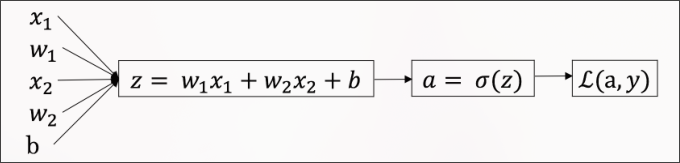
\includegraphics[width=0.8\linewidth]{figures/computational_graph}
  \end{center}
  \caption{Computational graph}\label{fig:computational graph}
\end{figure}

The first column are the inputs, the second column represents a neural network of type $z = w^T x + b$, in the third one is described the activation function $a$ which is a sigmoid ($\sigma$) and the fourth and final column is the output, represented by a loss function.

To improve the loss function we need to change the 3 parameters $w_1, w_2$ and $b$ and the new values of these parameters will be

\begin{align*}
  w_1 & \coloneqq w_1 - \alpha \diff{J(w,b)}{w_1} \\
  w_2 & \coloneqq w_2 - \alpha \diff{J(w,b)}{w_2} \\
  b & \coloneqq b - \alpha \diff{J(w,b)}{b}
\end{align*}

where $d$ is the derivative.
\\\\
For instance, if we have the following function loss
\begin{equation*}
  Cost(a,y) = \mathcal{L}(a,y) = - [y \cdot ln(a) + (1 - y) \cdot ln(1 - a)]
  \label{eq:}
\end{equation*}
the derivatives will be
\begin{align*}
  \diff{\mathcal{L}}{a} & = - \frac{y}{a} + \frac{1-y}{1-a} \\
  \diff{\mathcal{L}}{z} & = \diff{\mathcal{L}}{a} \cdot \diff{a}{z} = \left( - \frac{y}{a} + \frac{1-y}{1-a} \right) \cdot (a(1-a)) = - y + \cancel{ya} + a - \cancel{ya} = a - y\\
  \diff{\mathcal{L}}{w_1} & = \diff{\mathcal{L}}{z} \cdot \diff{z}{w_1} = (a-y)x_1 \\
  \diff{\mathcal{L}}{w_2} & = \diff{\mathcal{L}}{z} \cdot \diff{z}{w_2} = (a-y)x_2 \\
  \diff{\mathcal{L}}{b} & = \diff{\mathcal{L}}{z} \cdot \diff{z}{b} = (a-y) \cdot 1 = (a-y)
\end{align*}

Let us remember that the sigmoid function is $\sigma (x) = \frac{1}{1 + e^{-x}}$, thus its derivative is $\sigma^\prime (x) = \sigma (x) \cdot (1 - \sigma (z))$.

\subsection{Random initialization}

If we initialize the weights to zero, it happens that all the neurons will have an equal value and this is a problem called \textbf{symmetry problem}.
In fact, by initializing the weights to zero, each neuron in the first hidden layer will perform the same computation so, even after multiple iterations of gradient descent, each neuron in the layer will be computing the same thing as other neurons.
A possible solution to this problem is to make a random initialization of the weights.

Biases, instead, don't suffer for the same problem and can be initialized to zero.

\chapter{Neural Networks Improvements}

\section{Hyperparameters}

\begin{figure}[h]
  \begin{minipage}{0.6\linewidth}
    Hyperparameters are:
    \begin{itemize}
      \item learning rate
      \item number of epochs
      \item number of hidden layers
      \item number of hidden units (in each hidden layer)
      \item activation functions
    \end{itemize}
    All of these parameters are chosen empirically, following the cycle seen in \textit{figure~\ref{fig:hyperparameters}}
  \end{minipage}
  \hfill
  \begin{minipage}{0.35\linewidth}
      \begin{center}
        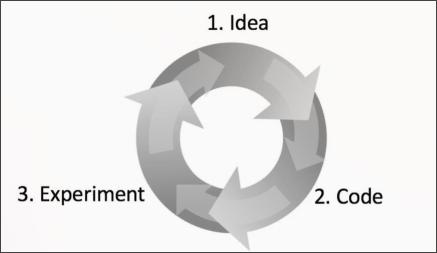
\includegraphics[width=\linewidth]{figures/hyperparameters}
      \end{center}
      \caption{hyperparameters empirical cycle}\label{fig:hyperparameters}
  \end{minipage}
\end{figure}

\section{Train/Dev/Test sets}

The following image represents the distribution of the dataset over the different phases.

\begin{figure}[h]
  \begin{center}
    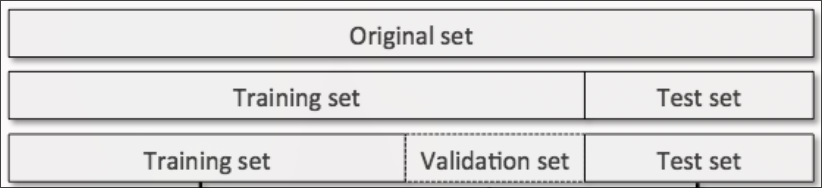
\includegraphics[width=0.7\linewidth]{figures/train_dev_test}
  \end{center}
\end{figure}

It's important that validation and test sets should come from the same distribution.

If the data set is small, we can enlarge it with other similar ``general'' data (for example taken from the web), but these data must be used only in the training set.
For instance, if we want to recognize cat photos taken with a smartphone, we can use ``general'' cat photos in the training set, but in the validation and test sets we must use only images taken with a smartphone.

\newpage

\section{Underfit/Overfit}

\textbf{underfit} = models don't have the capacity to fully learn the data.

\textbf{overfit} = too complex, doesn't generalize well.

\vspace{15pt}

\begin{figure}[h]
  \begin{center}
    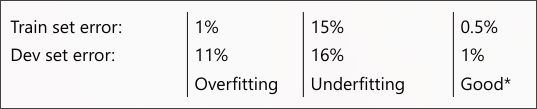
\includegraphics[width=0.7\linewidth]{figures/overunderfit_table}
  \end{center}
\end{figure}

\begin{figure}[h]
  \begin{center}
    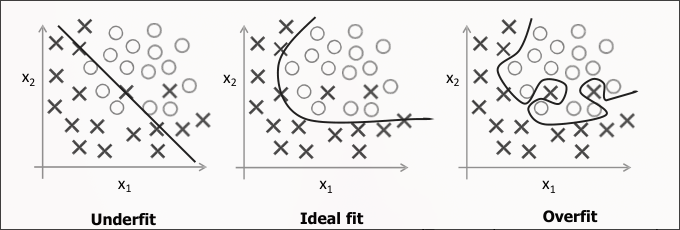
\includegraphics[width=\linewidth]{figures/overunderfit_graph}
  \end{center}
\end{figure}

As we can see from the two images above, overfitting is very precise, but even with a small change, it's performance decrease drastically.
In the other hand, underfitting is more balanced and stable during the training and verification phases, but has higher error values than the ideal (good) case.

To solve underfitting we can try to:
\begin{itemize}
  \item increase the network size, by making the network deeper or by increasing the number of units in each hidden layer
  \item prolong the training phase with additional epochs
\end{itemize}

Instead, to solve overfitting we can try to:
\begin{itemize}
  \item use more training data (not so easy, it's a cost in terms of money and time)
  \item use regularization (increase the regularization parameter lambda; in this way the weights are pushed toward becoming smaller, so closer to 0)
\end{itemize}

Neural networks are more flexible for reducing underfitting/overfitting problems than the traditional Machine Learning approaches.

\newpage

\subsection{Regularization}

The formula for the minimization problem with regularization is
\begin{gather}
  min_{(w,b)}\ J(w,b)
  \label{eq:regularization}
  \intertext{where the cost function $J(w,b)$ definition is}
  J(w,b) = \frac{1}{m} \left[ \sum_{i=1}^{m} \mathcal{L} \left(\hat{y}^i, y^i \right) + \frac{\lambda}{2} \sum_{j=1}^{n} w_j^2 \right]
  \label{eq:cost_in_regularization}
\end{gather}
and $\lambda$ is the \textbf{regularization parameter}.
The bias $b$ is ignored in regularization.
\\\\
The first part of the cost function formula (\ref{eq:cost_in_regularization}) is equal to the base one and its aim is to reach a final cost as close as possible to 0.
The second part instead, tries to regularize the weights (have weights as close as possible to 0), otherwise we will have problem in the loss.

If there are huge differences between the weights, there will be high chances that the activation function output will be based only on the big weights, while the small ones won't be considered.
This translates into having a subset of the original neural network with only the big weights, losing precious information from the small weights.
Regularization tries to avoid this scenario by using an average of the sum of the weights.

If we have multiple hidden layers then the second part of the formula will be instead
\begin{gather}
  + \frac{\lambda}{2} \sum_{l=1}^{L} \left\Vert W^{[l]} \right\Vert_F^2 
  \label{eq:cost_in_regularization_with_layers}
\end{gather}
where $l$ is the layer and
\begin{gather*}
  \left\Vert W^{[l]} \right\Vert_F^2 = \sum_{i=1}^{n^{[l-1]}} \sum_{j=1}^{n^{[l]}} \left( W_{ij}^{[l]} \right)^2
\end{gather*}

The term~\ref{eq:cost_in_regularization_with_layers} of the formula~\ref{eq:cost_in_regularization} with layers, is the sum of all the components that are in the weight's matrix.

The backpropagation with the regularization term is:
\begin{gather*}
  \diff{\mathcal{L}}{W^{[1]}} = \diff{\mathcal{L}}{z^{[1]}} \cdot x^T + \frac{\lambda}{m} \cdot W^{[1]}
\end{gather*}
where the second term is added because of the regularization and therefore is called \textbf{regularization effect}.

Regularization in neural networks is also called \textbf{weight decay}. In fact, it is a regularization technique (such as L2 regularization) that results in gradient descent shrinking the weights on every iteration.

\begin{gather*}
  \theta = \theta - \alpha \diff{J}{\theta}
\end{gather*}

\newpage

\subsection{Dropout regularization}

It's a common overfitting solution and this technique consists in \textbf{randomly ignoring} (or ``dropping out'') some neurons in the hidden layers in order to \textbf{train} the model with a \textbf{smaller} network.
This behavior makes the training process \textbf{noisier}, forcing nodes within a layer to probabilistically take responsibility of the input.
This technique is effective because it randomly forces the nodes, to avoid big nodes from abusing the model.

The dropout can only be used in the training because in the other phases it's needed the whole network.

Usually are used higher probabilistic values (stronger dropout) in the first layers and lower values in the last ones, \textit{i.e.} the dropout value is lowered as much as close we are to the output layer of the network.

\subsection{Data augmentation}

Data augmentation, in data analysis, are techniques used to increase the amount of data by adding slightly modified copies of already 
existing data or newly created synthetic data from existing data.
The typical transformations are
\begin{itemize}
  \item geometric transformations
  \item flipping
  \item color modification
  \item cropping
  \item rotation
  \item noise injection
  \item random erasing
\end{itemize}

\subsection{Early stopping}

\begin{figure}[h]
  \begin{minipage}{0.6\linewidth}
    When having a large network, there will be a point during training when the model will stop generalizing and start learning the statistical noise in the training dataset.

    This overfitting of the training dataset will result in an increase in generalization error, making the model less useful at making predictions on new data.
  \end{minipage}
  \hfill
  \begin{minipage}{0.35\linewidth}
      \begin{center}
        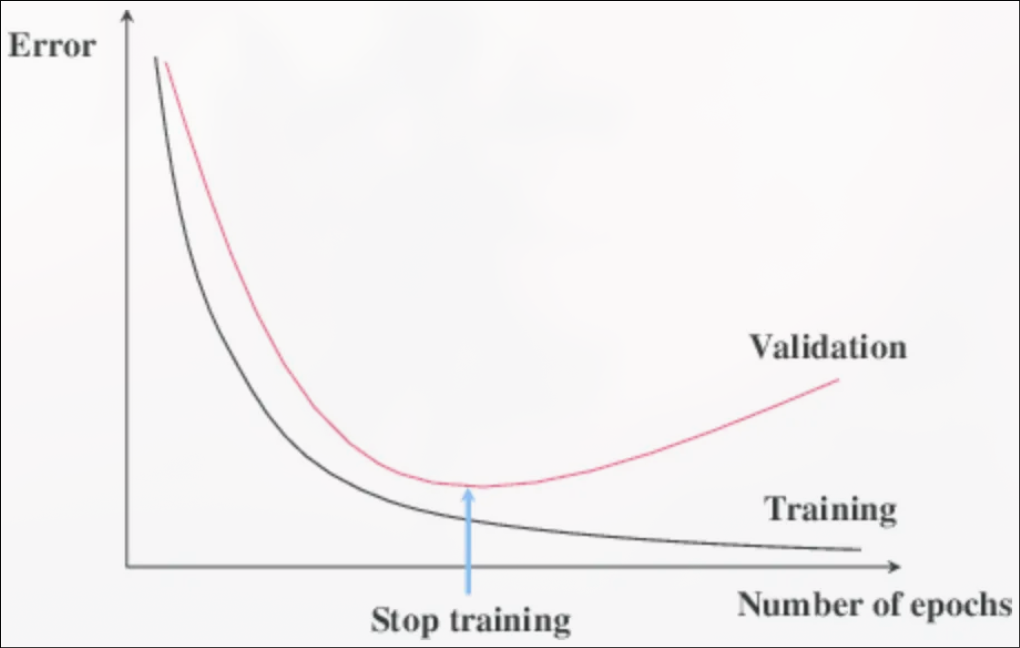
\includegraphics[width=\linewidth]{figures/early_stopping}
      \end{center}
  \end{minipage}
\end{figure}

One approach to solve this problem is to treat the number of training epochs as a hyperparameter and train the model multiple times with different values, then select the number of epochs that returned the best performance.

\section{Normalization}

\subsection{Mean Normalization}

It’s the preferred normalization for Neural Networks, and it transforms data to have a mean $\mu = 0$ and a standard deviation $\sigma = 1$.
Given a feature $x_i$ the mapped feature is 
\begin{equation*}
  x_i^\prime = \frac{x_i - \mu_i}{\sigma_i}
\end{equation*}
where $\mu_i$ and $\sigma_i$ area both computed on the training set and are respectively

\begin{definition}[Mean]
  \begin{equation*}
    \mu_i = \frac{1}{m} \sum_{i=1}^{m} x_i
  \end{equation*}
\end{definition}

\begin{definition}[Standard deviation]
  \begin{equation*}
    \sigma_i = \sqrt{\frac{1}{m-1} \cdot \sum_{i=1}^{m} (x_i - \mu_i)^2}
  \end{equation*}
\end{definition}
where $m$ is the number of samples of the training set.

\subsection{MinMax Normalization}

This normalization shifts the data such that all features are exactly between 0 and 1.
\begin{equation*}
  x_i^\prime = \frac{x_i - \min(x)}{\max(x) - \min(x)}
\end{equation*}

$x_i$ is the original value and $x_i^\prime$ is the normalized one.

\subsection{Comparison}

In the following image we can see a comparison between the two types of normalization, where the Mean is called StantardScaler and MinMax is the MinMaxScaler.

\begin{figure}[h]
  \begin{center}
    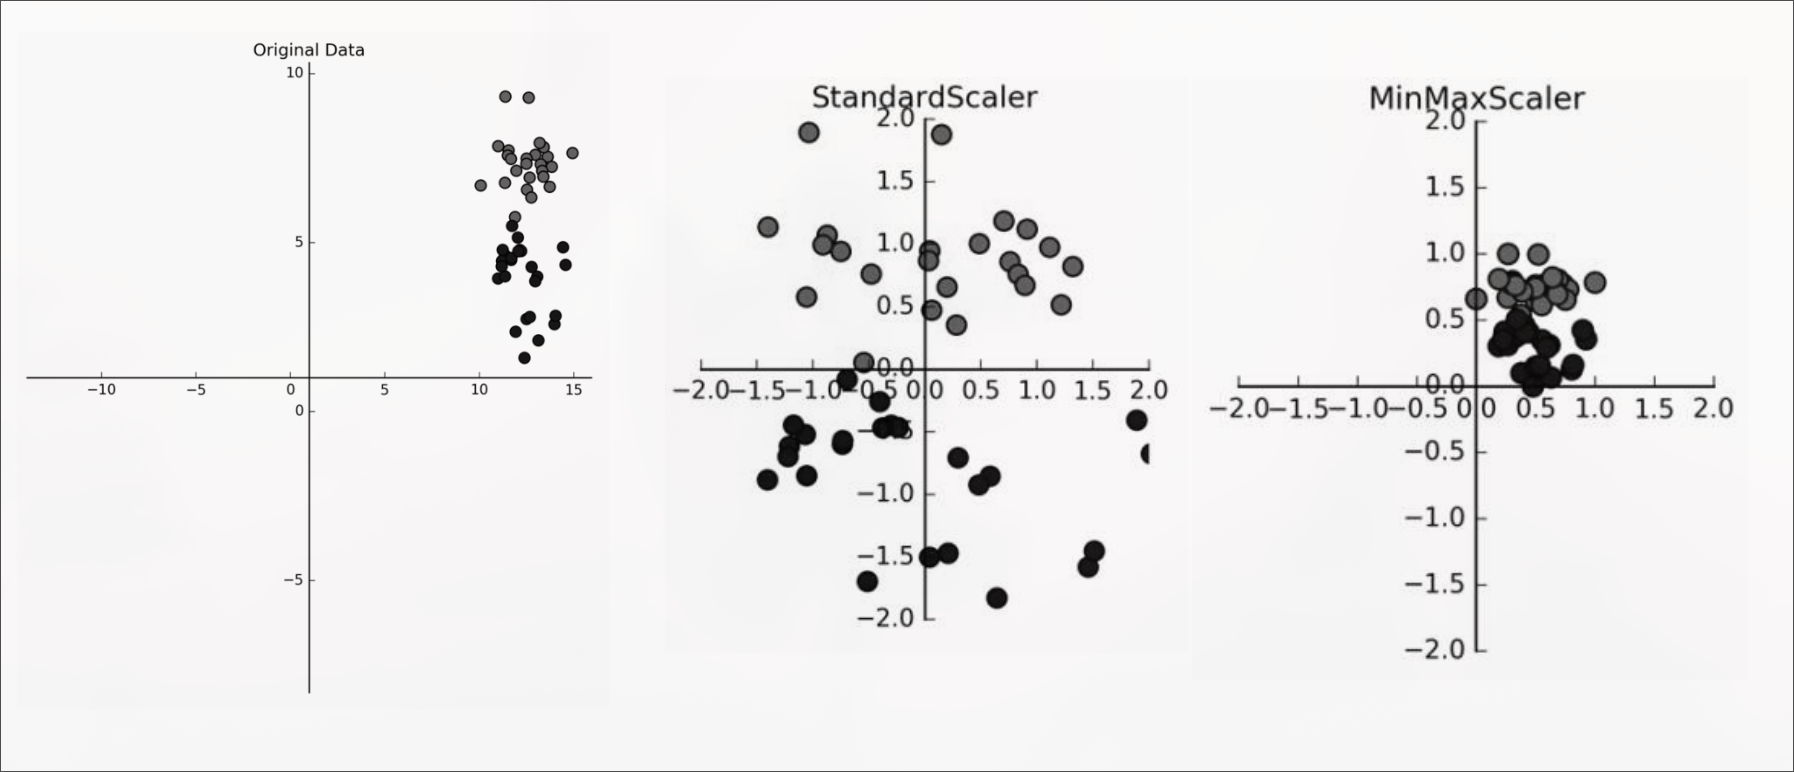
\includegraphics[width=0.65\linewidth]{figures/normalization_comparison}
  \end{center}
\end{figure}

It's important to use the \textbf{same transformation} both for the training and the test, otherwise we could end up with two different scalings between the training and the test, like in the example in \textit{Figure~\ref{fig:normalization_example2}}.

\begin{figure}[h]
  \begin{minipage}{0.48\textwidth}
    \centering
    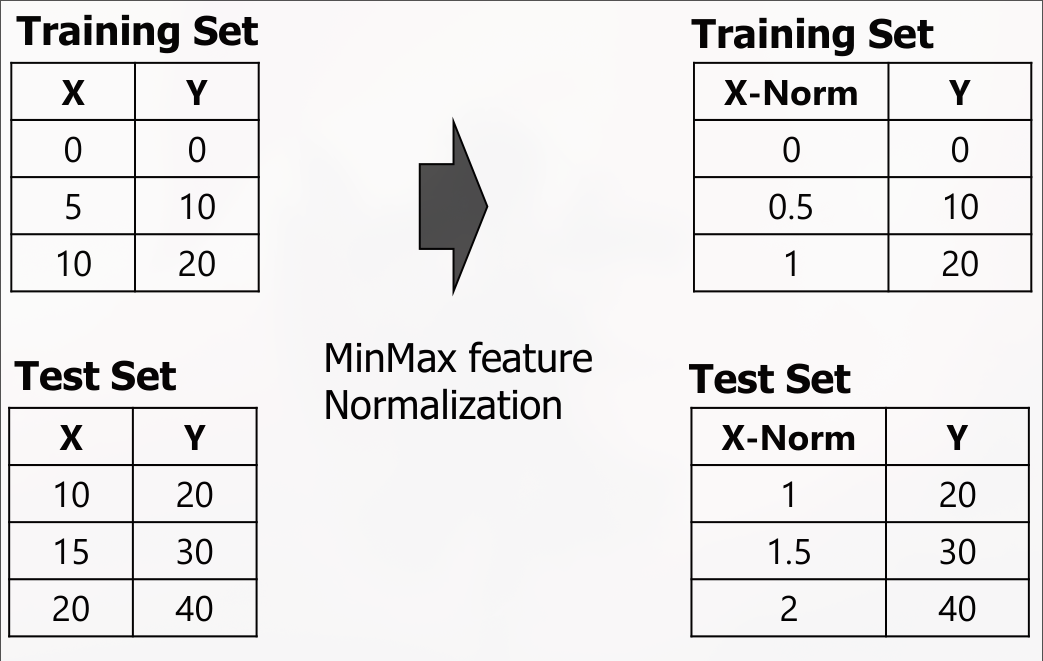
\includegraphics[width=\linewidth]{figures/normalization_example1}
    \caption{Correct transformation}\label{fig:normalization_example1}
  \end{minipage}
  \hfill
  \begin{minipage}{0.48\textwidth}
    \centering
    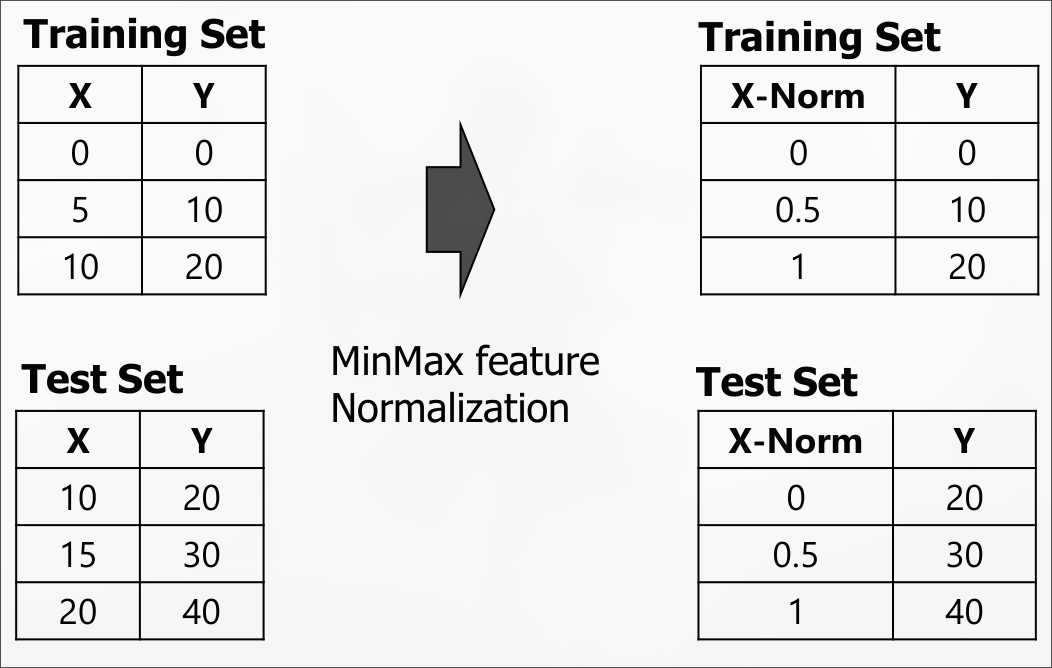
\includegraphics[width=\linewidth]{figures/normalization_example2}
    \caption{Incorrect transformation}\label{fig:normalization_example2}
  \end{minipage}
\end{figure}

As you can see, in \textit{Figure~\ref{fig:normalization_example1}}, has been used the \textbf{same values} ($\min=0$ and $\max=10$), while in \textit{Figure~\ref{fig:normalization_example2}} for the training has been used $\min=0$ and $\max=10$ and for the test $\min=10$ and $\max=20$.
We can see immediately the difference, because the \textbf{same tuple} (10,20) of the dataset, has been scaled in two \textbf{different mappings} (1,20) and (0,20).
\\\\
With normalized inputs the \textbf{gradient descent} will perform better, finding the minimum \textbf{efficiently}, as we can see in the image below, where the arrows represent the path followed by the gradient descent algorithm in order to find the minimum.

\begin{figure}[h]
  \begin{center}
    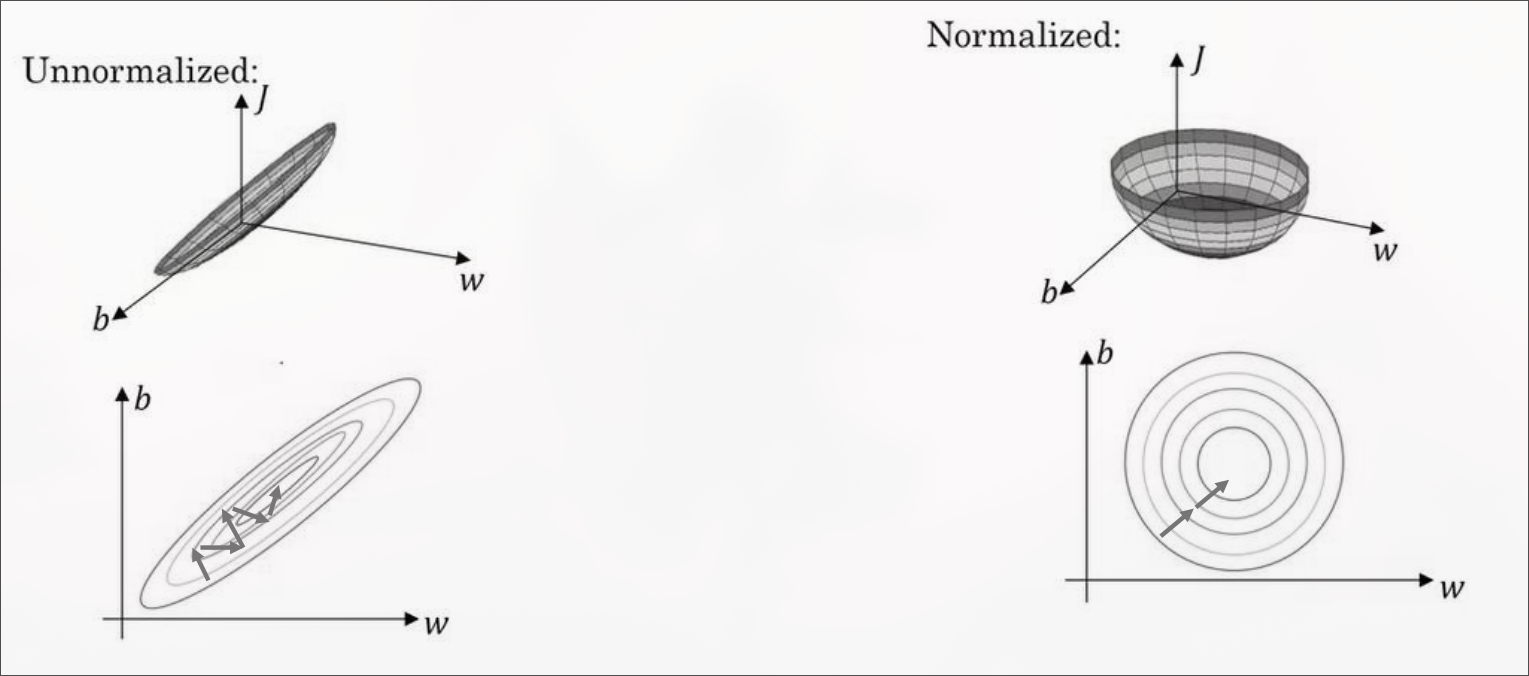
\includegraphics[width=0.7\linewidth]{figures/why_normalize}
  \end{center}
\end{figure}

\section{Vanishing/Exploding Gradients}

Let's suppose we have a net with $g^{[i]}(z) = z$, $b^{[i]} = 0$ and $L$ hidden layers, all equal to each other, for example $\begin{bsmallmatrix} 1.5 & 0 \\ 0 & 1.5 \end{bsmallmatrix}$, then the output will be $\hat{y} = \begin{bsmallmatrix} 1.5 & 0 \\ 0 & 1.5 \end{bsmallmatrix}^L$, which will have really large values.
Instead, if the layers where equal to $\begin{bsmallmatrix} 0.5 & 0 \\ 0 & 0.5 \end{bsmallmatrix}$, then the output will have small values.
To resolve this problem, a solution is to set randomly the weights around 1.

\chapter{CNN - Convolutional Neural Networks}

\section{Computer Vision}

In this field there are a lot of subfields, all related to the manipulation of data contained in images, for example:
\begin{itemize}
  \item \textbf{image classification} - recognize if an image contains a specific object in order to classify it ``\textit{Does this image contain a cat? Yes/No}''
  \item \textbf{object detection} - find all the occurrences of an object in an image ``\textit{Find cars in the image}''
  \item \textbf{action recognition} - from a sequence of images recognize the ongoing action ``\textit{What is the person doing?}''
  \item \textbf{captioning} - brief textual description of the image ``\textit{A boy holding a toy hammer}''
\end{itemize}

\textbf{SAM} is a system able to segment images.
This type of recognition is fundamental in the field of image generation/manipulation, because, with an image divided in segments, it is possible to replace only a specific segment of it (e.g. the segment of the subject or the segment of the background).

An image is a \textbf{tensor} (matrix) of integers in the range [0, 255] where each number is a channel of the RGB\footnote{Red Green Blue} color-space of a specific pixel. For instance, with a colored image of $800 \times 600$ pixels, the quantity of integers needed to represent the photo in a computer is $800 \times 600 \times 3$.

The main challenges for image detection are:
\begin{itemize}
  \item \textbf{viewpoint variation} - even with a slight move in space of the camera, means that all the pixels change, so a totally different tensor, but a neural network model must be able to recognize the object anyway
  \item \textbf{background clutter} - this problem arises when the background has a chromatic gamma similar to the one of the subject (e.g. white cat in the snow)
  \item \textbf{illumination} - different light means that the camera records the colors differently, thus we have a complete different sets of pixels, even with the same exact position of the camera, object and environment, but just a different type of light (e.g. day vs night)
  \item \textbf{context} - also the context/environment around the subject and the position of it in the environment means different results
  \item \textbf{deformation} - for instance, a person can stay in different positions, and each one is a complete different image
  \item \textbf{intraclass variation}
\end{itemize}

\section{Convolutional filter}

Working on large images, for instance an HD picture that has $1920 \times 1080$ pixels ($1920 \times 1080 \times 3 > 6$ millions values), it becomes impossible using standard neural networks that we have seen until now, because, suppose that we have a small hidden layer of just 1000 weights, it means that there are over 6 billions edges between the input and the first hidden layer.
\\\\
To solve this problem are born different solutions and for example, to recognize objects, a possible one is to work on the edges of the shapes present in the image.
As we can see in the image below, we can extract only the data of the vertical (or horizontal) edges.

\begin{figure}[h]
  \begin{center}
    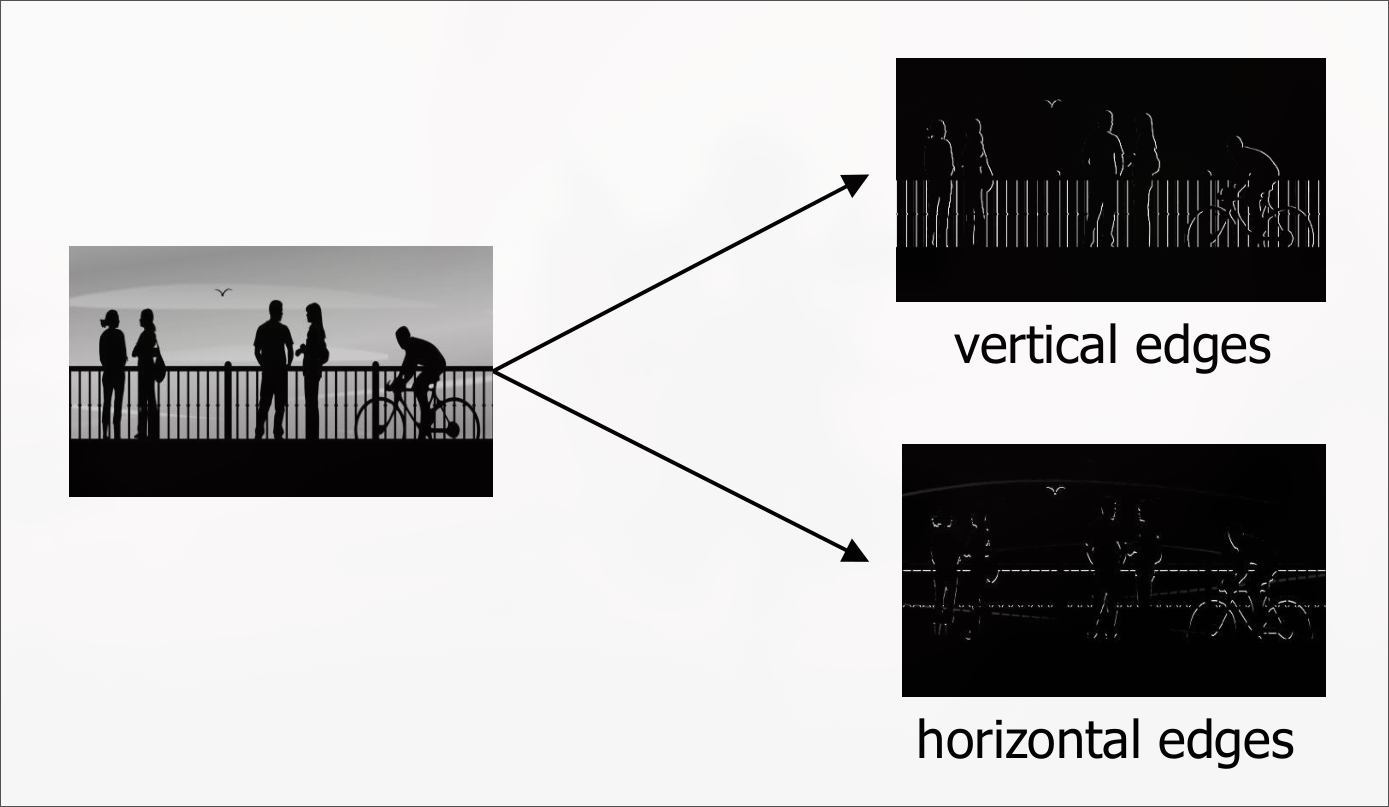
\includegraphics[width=0.6\linewidth]{figures/edges}
  \end{center}
\end{figure}

To do so, are used \textbf{convolutional filters}, which are matrixes with fixed values, depending on the result we want to obtain.
Given the input data mapped into a matrix and a filter, the convolution is the output matrix of their inner product. The formula used to obtain the convolution is:
\begin{equation*}
  I(x,y) \cdot h = \sum_{i=-a}^a \sum_{j=-b}^b I(x-i, y-j) \cdot h(i,j)
\end{equation*}
where multiplication contained in the two nested sums is called \textbf{inner product}.

\begin{figure}[h]
  \begin{center}
    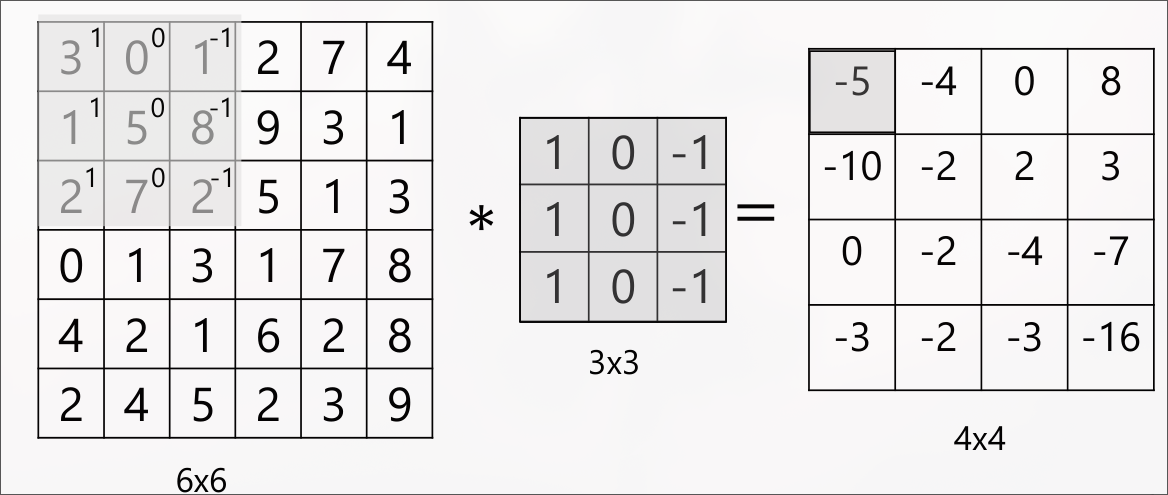
\includegraphics[width=0.55\linewidth]{figures/convolution}
  \end{center}
  \caption{Example of convolution}
\end{figure}

The matrix on the left is composed of the input data (the data of the image), the small matrix in the center is the filter and the one on the right is the convolutional output.

The filter $\begin{bsmallmatrix} \ 1 & 0 & -1 \\ \ 1 & 0 & -1 \\ \ 1 & 0 & -1 \end{bsmallmatrix}$ is specialized to detect if there is a \textbf{vertical} edge in the input, while to detect \textbf{horizontal} edges is used the filter $\begin{bsmallmatrix} \ 1 & \ 1 & \ 1 \\ \ 0 & \ 0 & \ 0 \\ -1 & -1 & -1 \end{bsmallmatrix}$.

In the image below there are other examples of filters for image manipulation

\begin{figure}[h]
  \begin{center}
    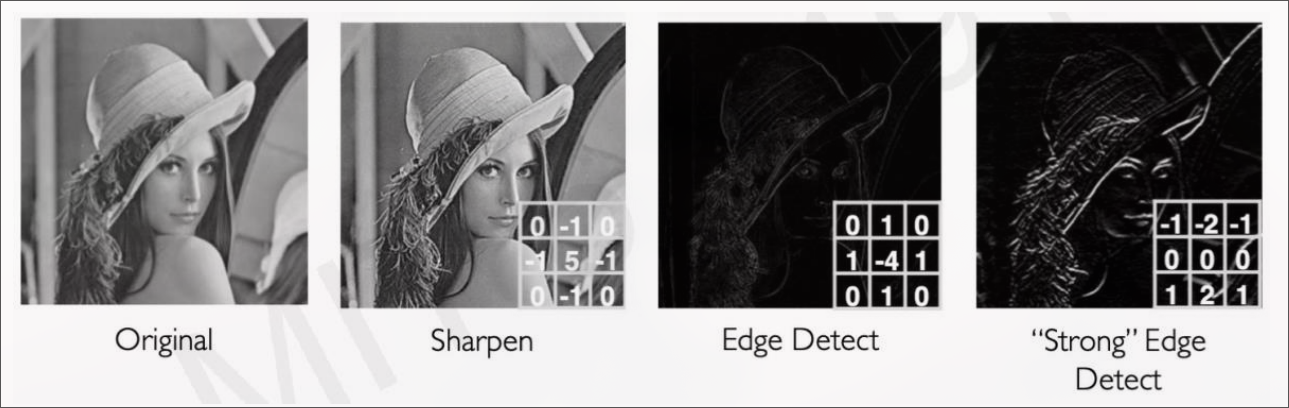
\includegraphics[width=0.9\linewidth]{figures/image_manipulation_filters}
  \end{center}
  \caption{Examples of filters}
\end{figure}

Image processing and Computer Vision has many handcrafted filters like Canny, Sobel, Gaussian Blur, Morphological filters, Gabor Filters, etc...

\subsection{Padding}

Given a matrix input of size $n$ and a filter of size $m$, the convolutional output matrix will be of size $n - m + 1$, which is equal to $n$ only if the filter has size 1.
In all the other cases the output matrix will be smaller and in most situations this is not a problem, but sometimes the model need a matrix of the same size.
To solve this problem, has been invented the \textbf{padding} technique, which consists in adding $k \ge 0$ external layers of 0s around the original matrix, where $k = \frac{m - 1}{2}$.
In the example below, we can see that we had an input of $6 \times 6$ and a filter of $3 \times 3$, but the output would have been a $4 \times 4$ matrix, so, to keep the original size in the output, we added $k = \frac{3 - 1}{2} = 1$ line of 0s all around the original matrix.

\begin{figure}[h]
  \begin{center}
    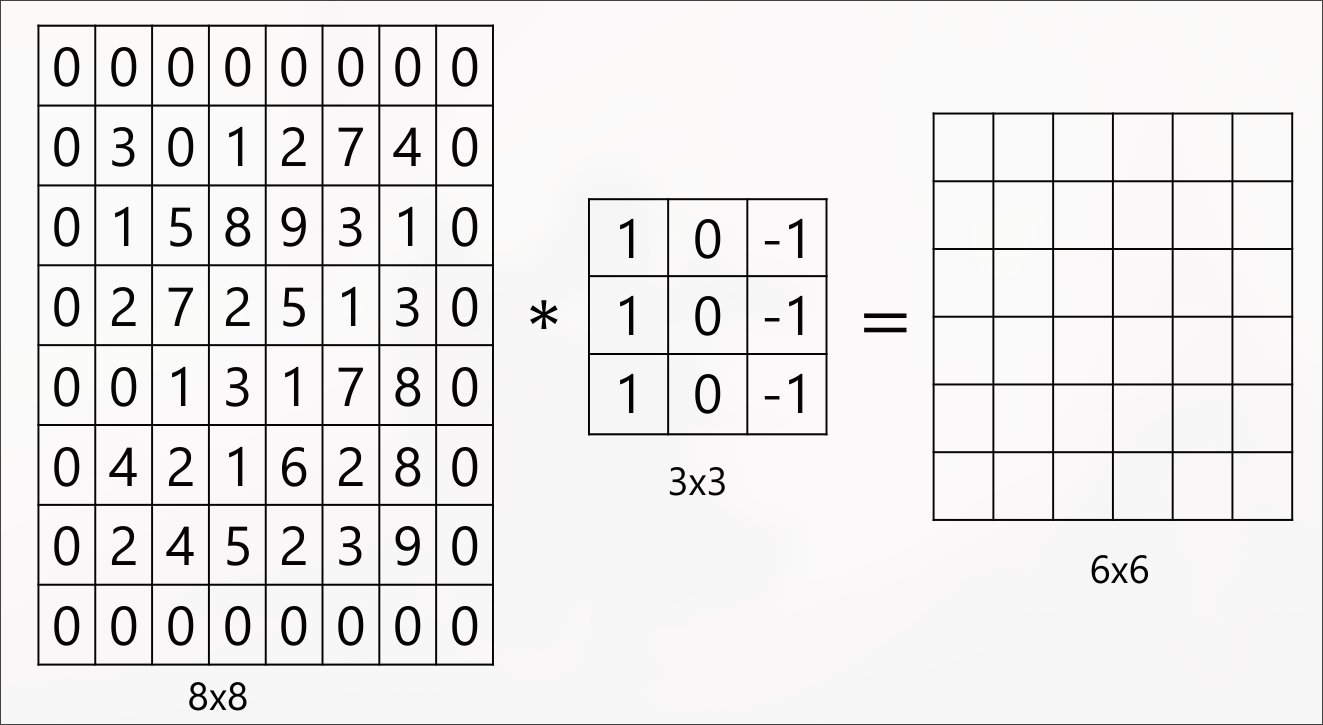
\includegraphics[width=0.6\linewidth]{figures/padding}
  \end{center}
\end{figure}

\newpage

\subsection{Strided Convolution}

Sometimes when we have an image with a very big amount of pixels and those are also very similar to each other (have close values), while calculating the convolution, instead of moving of only 1 pixel at a time, we can set a \textbf{stride}, which corresponds to the number of pixels we need to move while calculating each cell of the convolution.
Obviously the output matrix will have an even smaller size than the input, so it does pretty the opposite of the padding.

\begin{figure}[h]
  \begin{center}
    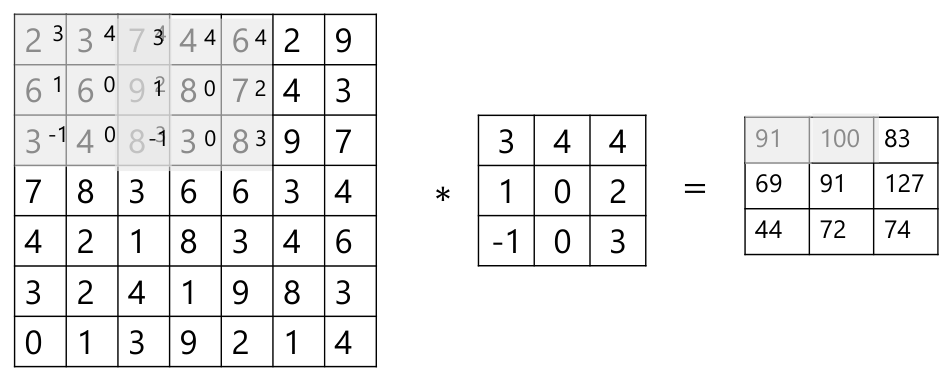
\includegraphics[width=0.6\linewidth]{figures/stride}
  \end{center}
  \caption{Example with stride=2}
\end{figure}

If we have an input matrix, where we have a stride that makes us go outside of it and not matching perfectly in the last columns, then we simply skip that convolution and proceed on a new line (if possible, otherwise we stop).
For example, if in the above image we had set the stride to 3, then we will have covered columns from 1 to 3 in the first step, 4 to 6 in the second and in the last one we would have had only the 7th column, but we needed a total of three to go on, so we skip that and start a new line.

\subsection{Multi-layered Convolution}

If we have multiple layers in the input matrix, the convolutional filter must have the same number of layers.
For instance, if we work with colored images, these will be represented as a matrix of 3 layers (one for each RGB channel), so also the filter must be a 3-layered matrix.

\begin{figure}[h]
  \begin{center}
    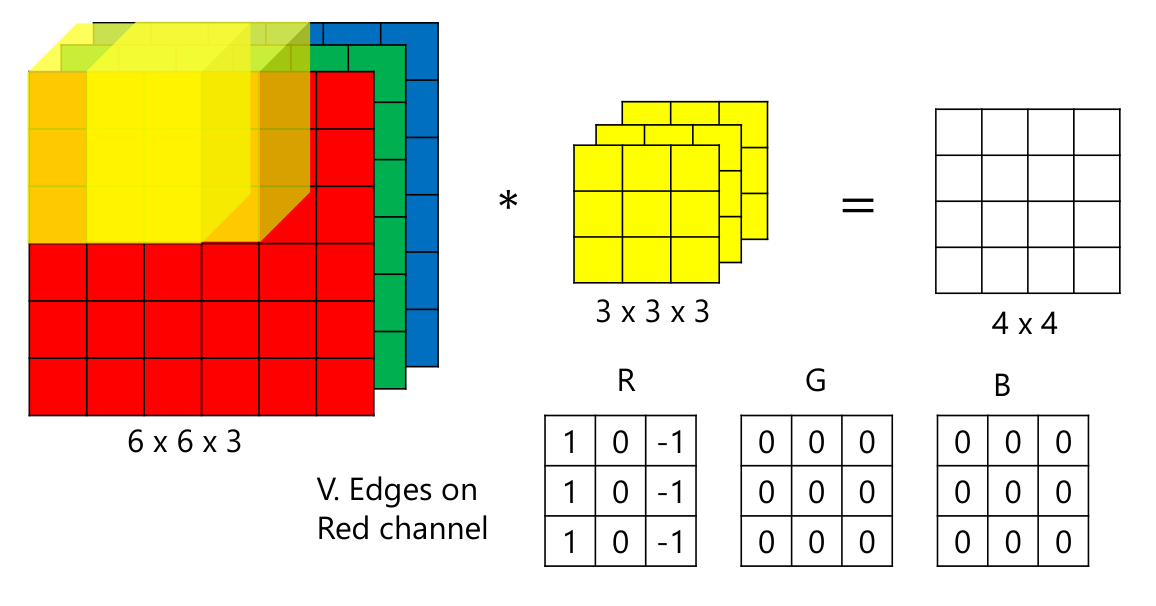
\includegraphics[width=0.6\linewidth]{figures/RGB_convolution}
  \end{center}
  \caption{Example of RGB convolution}
\end{figure}

As we can see in the image, the output is a single layer matrix, so the image represented by that matrix will have only 1 channel.

\newpage

\section{Convolutional Layers}

Are convolutions applied to entire neural networks.
The network is equal to one with a traditional approach, but the number of edges is lower.
A convolutional layer is a network with one or more filters, where the bias is applied to each convolutional output and then is also applied an activation function (often ReLU).
In these networks, edges are less because not all nodes are connected together, but only those reachable within the filter size (and the stride).

\begin{figure}[h]
  \begin{center}
    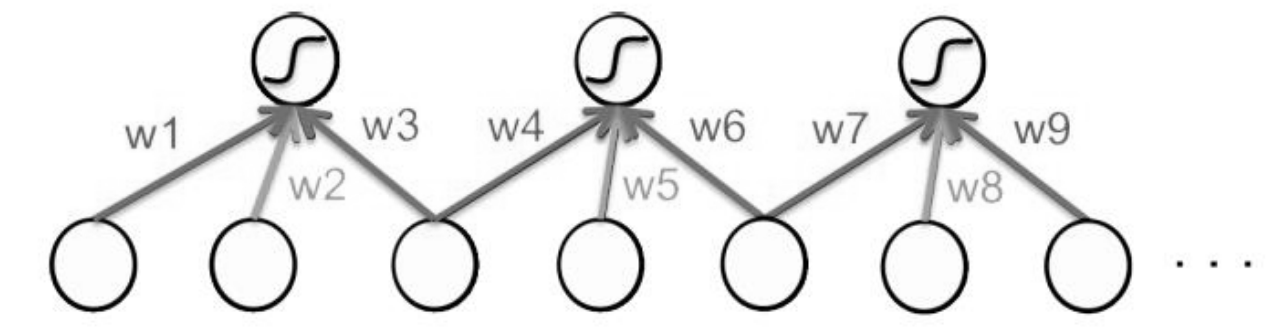
\includegraphics[width=0.5\linewidth]{figures/convolutional_layer}
  \end{center}
  \caption{Example of a convolutional layer with a filter of size $3 \times 3$ and stride $=2$}\label{fig:convolutional layer}
\end{figure}

Convolutions reduce dimensionality, in fact, by applying convolutional layers, the images get smaller and smaller (e.g. in the image, after only two convolutional layers, the information is reduced to only 1 pixel) and this means losing details so the recognition accuracy drops. 

Given two dataset S and T, where the first is fully annotated and plenty of images but not specific for our task, while the second is small but is precise for what we're looking for, we can build a model $h_S$ and use it to make the model $h_T$ learn better. This process is called \textbf{transfer learning}.

\subsection{Backpropagation with convolutions}

Let's suppose we are working on the same example of \textit{Figure~\ref{fig:convolutional layer}}, then the back propagation algorithm will work like this:
\begin{itemize}[label=]
  \item \textbf{forward pass} performs specific computations with all the weights $w_1, w_2, \dots, w_9$
  \item \textbf{backward pass} first compute the gradients $\frac{\partial J}{\partial w_1} , \dots , \frac{\partial J}{\partial w_9}$ for all the weights and then update the weights using the average of the gradients from the shared weights
    \begin{gather*}
      w_1 = w_1 - \alpha \left(\frac{\partial J}{\partial w_1} + \frac{\partial J}{\partial w_4} + \frac{\partial J}{\partial w_7} \right) \\
      w_4 = w_4 - \alpha \left(\frac{\partial J}{\partial w_1} + \frac{\partial J}{\partial w_4} + \frac{\partial J}{\partial w_7} \right) \\
      w_7 = w_7 - \alpha \left(\frac{\partial J}{\partial w_1} + \frac{\partial J}{\partial w_4} + \frac{\partial J}{\partial w_7} \right)
    \end{gather*}
\end{itemize}

\begin{note}
  $w_1, w_4 \text{ and } w_7$ because are on the same Red channel, so must be seen as a whole.
\end{note}

\newpage

A convolutional layer must have set all the convolutional parameters (filter size, padding, stride and number of filters).
\\\\
There exists multiple types of layer in Convolutional Networks, like:
\begin{itemize}
  \item Convolution (just seen)
  \item Pooling
  \item Fully connected (other name to call standard NN)
\end{itemize}

\section{Pooling Layer}

\subsection{Max Pooling}

It's a simple operation to reduce the size of the input. Given some parameters (the same for convolution), we split the input using those values and then, for each section we just take the maximum value. 

\begin{figure}[h]
  \begin{center}
    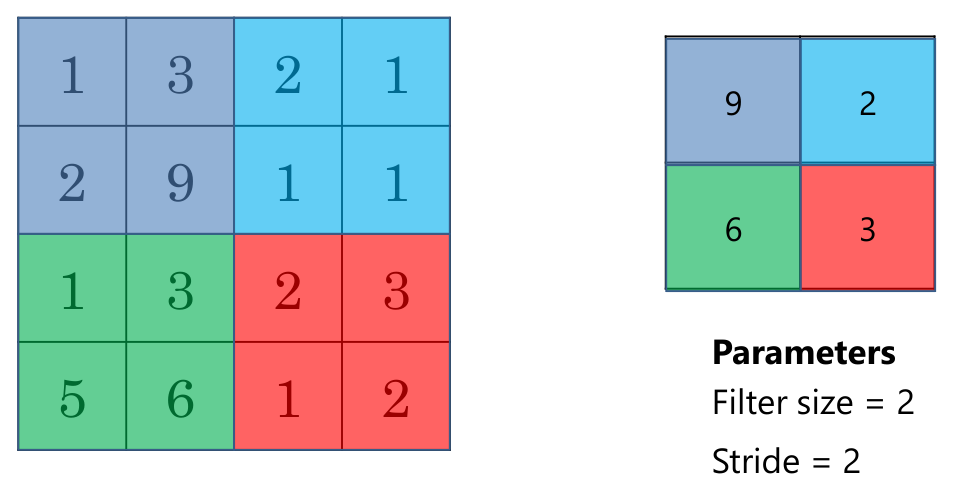
\includegraphics[width=0.45\linewidth]{figures/max_pooling}
  \end{center}
  \caption{Example of Max Pooling}
\end{figure}

This layer, like said before, is used only to reduce the size (for example we only want to do a simple classification, and we don't need all the pixels, so we speed up the procedure by reducing a little bit the size of the image), because are used no weights or bias, thus the model doesn't learn.

Usually this layer is used after a convolution and that's the reason why we take only the max value.
The idea of using this layer is to preserve the most important activation region (set of points) where the convolution filter found the most relevant points of the image.
\\\\
With multiple layers, the pooling filter is applied on each channel independently.
\\\\
Using a max pooling with a filter of size $2 \times 2$ and stride=2, is like doing the square root of the matrix input area, so dividing each size by 2, e.g. with an input matrix of size $32 \times 32 \times 28$, this max pooling layer will output a $16 \times 16 \times 28$ matrix.

\newpage

\section{Transfer Learning}

Even if we have a dataset T which is not large, we can train a CNN for it without overfitting.
We achieve this by pre-training a network over a dataset S, and then we can use:
\begin{itemize}
  \item \textbf{fine-tuning}: start the training over T with the same weights and network obtained by the training over S.
    It's better to use this if S is large and T is medium, because if there are too few data it's better to fine-tune only the last layers (the fully connected layers), while if there are more data we can fine-tune also the convolutional layers.
  \item \textbf{CNN as feature extractors}: used when the dataset T is very small and the extracted features are used as input for a classifier.
    Taking a feature means removing the last output layer from the CNN network, giving in input the dataset T, and then we use the output vectors of the CNN as input for a classifier.
\end{itemize}

\section{Modern Convolutional Networks Examples}

In convolutional networks we usually see
\begin{itemize}
  \item Multiple convolutional layers followed by a pooling layer.
  \item Fully-Conntected layers in the last few layers.
\end{itemize}

\subsection{AlexNet}

Was a really popular Neural Network, until some years ago.

\begin{figure}[h]
  \centering
  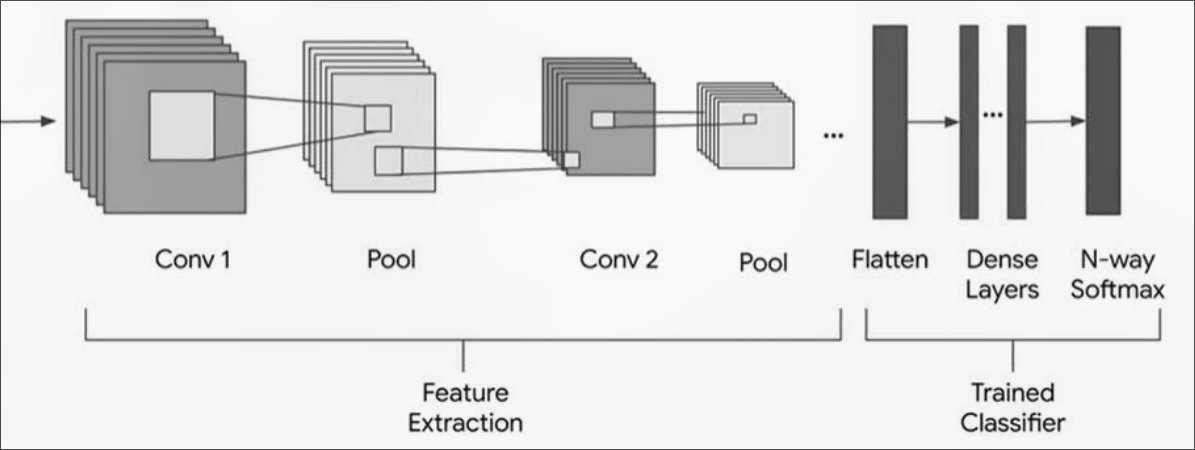
\includegraphics[width=0.75\linewidth]{figures/alexnet_architecture2}
  \\\vspace{10pt}
  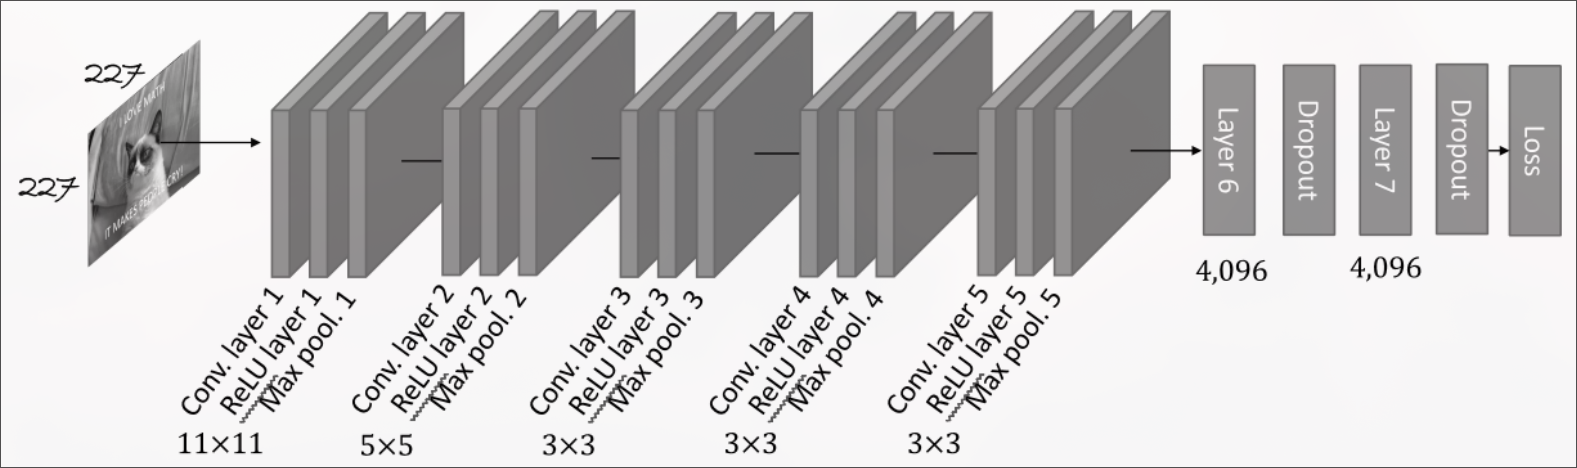
\includegraphics[width=0.9\linewidth]{figures/alexnet_architecture}
  \caption{AlexNet architecture}
\end{figure}

The convolutional layers are the fundamental part of the network, removing one of these translates into a big drop in performance, with only a small reduction of parameters (3\% drop, 1mln of parameters less).
In the opposite, removing one or either the last two fully-connected layers, isn't a big problem in terms of performance (1.6/5\% drop, but 16/50mln of fewer parameters).


\subsection{VGG16}

Is a network developed by the University of Oxford, which has achieved better results than AlexNet on image recognition (7.3\% vs 18.2\% of error rate).

\begin{figure}[h]
  \centering
  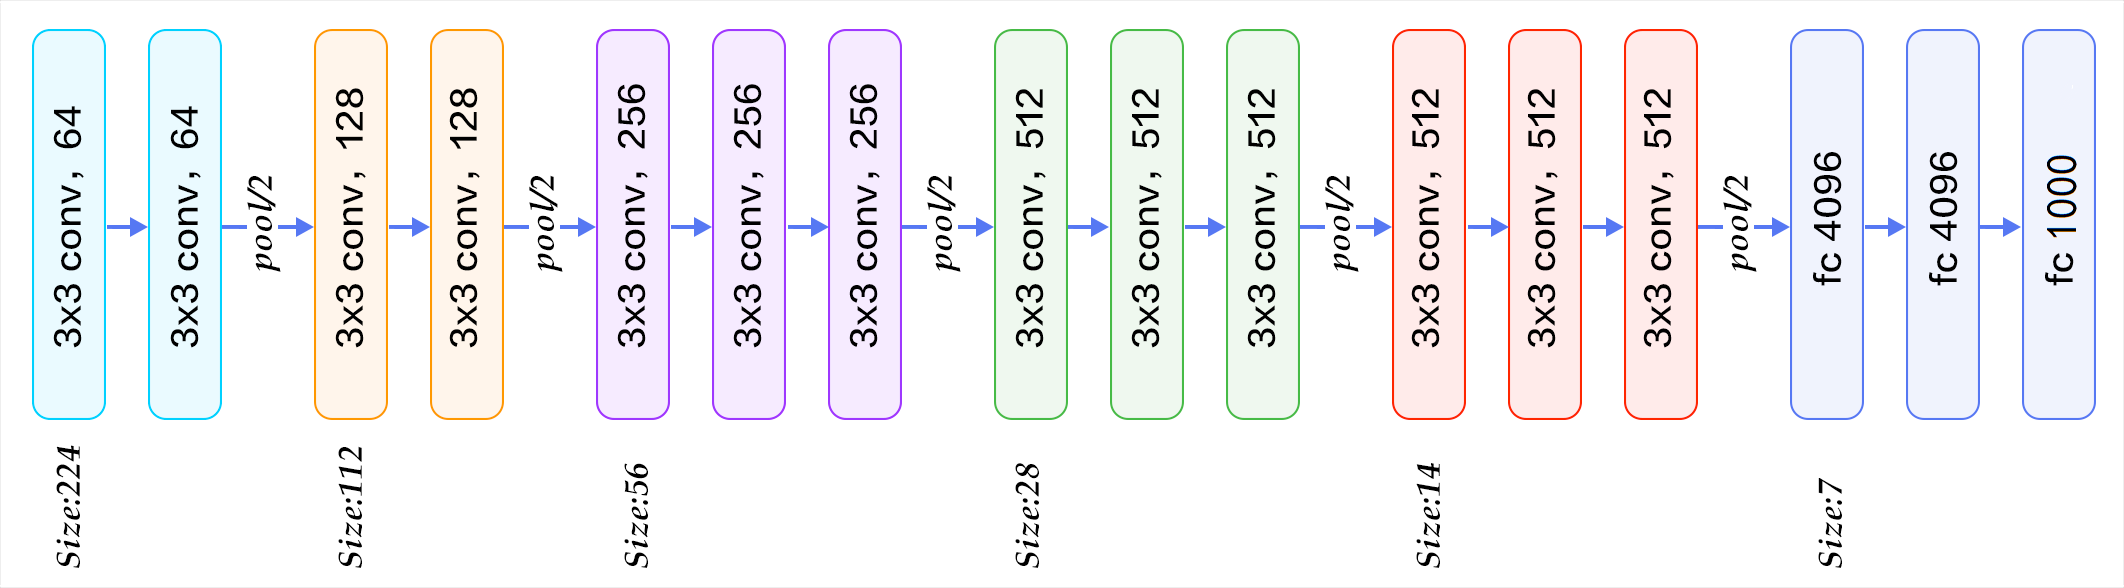
\includegraphics[width=0.9\linewidth]{figures/vgg16}
\end{figure}

In the network are used only $3 \times 3$ filters.
Two $3 \times 3$ filters have the receptive field of one $5 \times 5$ filter, while three $3 \times 3$ of a $7 \times 7$ filter.
However, using deeper stacks of smaller filters is more powerful than using a single larger filter and also generates fewer parameters (3 filters of $3 \times 3$ generates $3 \cdot 3 \cdot 3 = 27$ parameters, while a single $7 \times 7$ generates 49 parameters).

Furthermore, because for each convolutional filter we have an activation function, having several convolutional filters means having a deeper network that adds non-linearity into the system.

\subsection{Residual Networks}

With residual networks, we're able to design very deep neural networks.

In the two images below, we can see the visual difference between blocks of plain network and a residual one:

\begin{figure}[h]
  \centering
  \begin{minipage}{0.34\textwidth}
    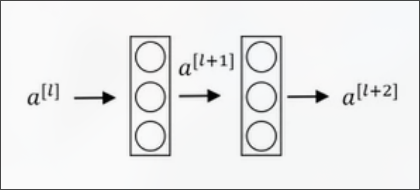
\includegraphics[width=\linewidth]{figures/plain_net}
    \caption{Plain}
  \end{minipage}
  \hfill
  \begin{minipage}{0.62\textwidth}
    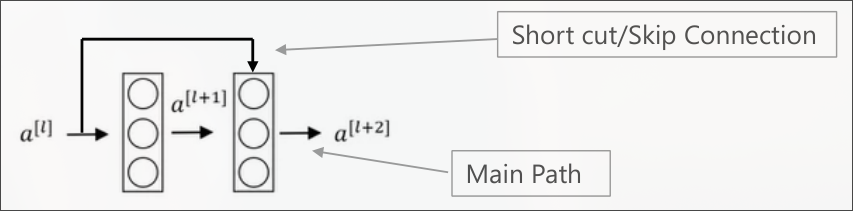
\includegraphics[width=\linewidth]{figures/resnet}
    \caption{Residual}
  \end{minipage}
\end{figure}

In the plain network we have that the value of $a^{\left[ l+2 \right]} = g(z^{\left[ l+2 \right]})$, while in the ResNet the formula slightly change into $a^{\left[ l+2 \right]} = g(z^{\left[ l+2 \right]} + a^{\left[ l \right]})$, where $z^{\left[ l+2 \right]} = W^{\left[ l+2 \right]} \cdot a^{\left[ l+1 \right]} + b^{\left[ l+2 \right]}$
\\\\
In the images below we can first compare two graphs that represents how the error rate change with the number of layers, and in the second comparison how are represented two real networks.

\begin{figure}[h]
  \centering
  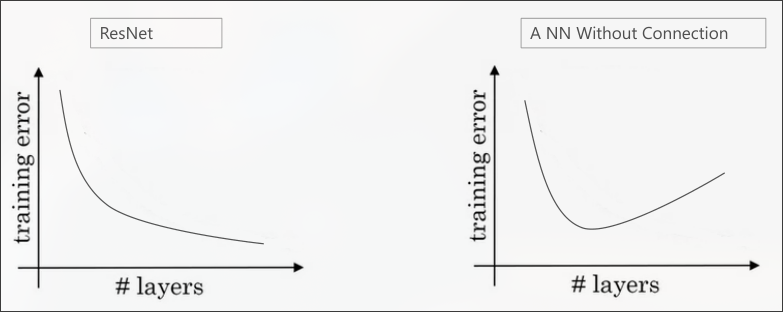
\includegraphics[width=0.45\linewidth]{figures/res_plain_difference_1}
\end{figure}

\begin{figure}[h]
  \centering
  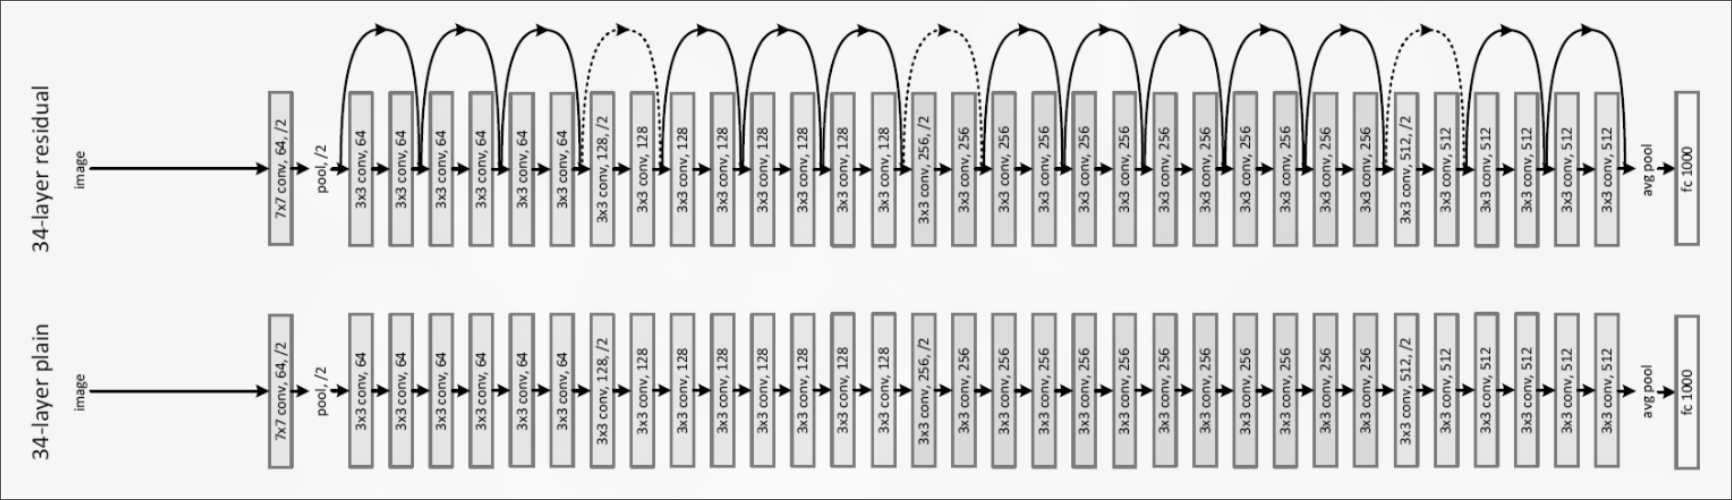
\includegraphics[width=\linewidth]{figures/res_plain_difference_2}
\end{figure}

With Max pooling we're able to decrease the size of a single channel.
If we want to reduce the number of channels we can use a $1 \times 1$ convolution.

\begin{figure}[h]
  \centering
  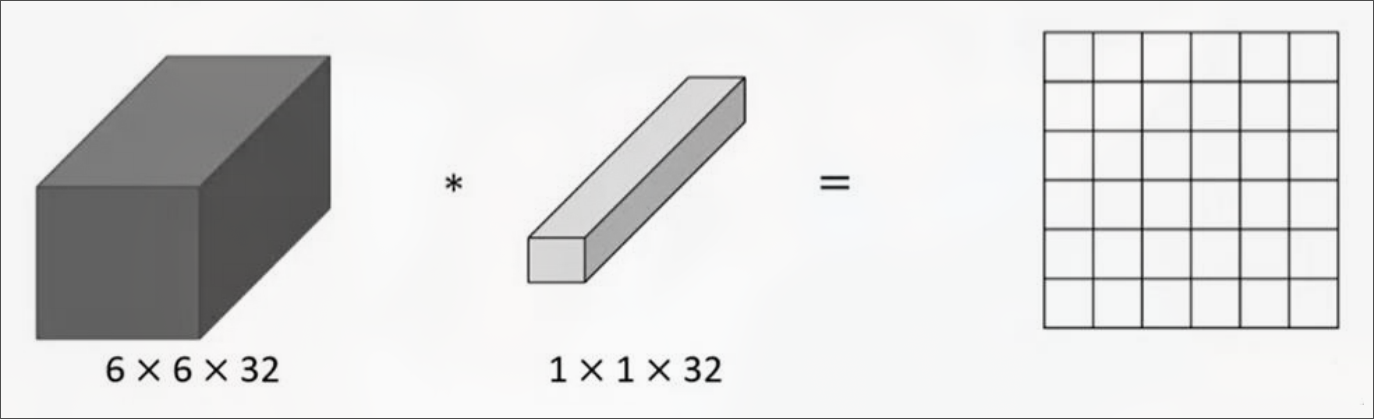
\includegraphics[width=0.5\linewidth]{figures/channel_reduction}
\end{figure}

As we can see in the figure above, the output is a 2D matrix ($6 \times 6 \times 1$) and the channels has been reduced from 32 to 1.

If we wanted to generate an output that were $6 \times 6 \times 5$, we would have needed to use 5 convolutional layers of dimensionality $1 \times 1 \times 32$.
These filters add also no-linearity factors.

We can achieve the same result of using multiple $1 \times 1$ filters, by using a single larger filter, but this means that the computational cost increases, because we have more multiplications to do.

\vspace{15pt}
\begin{minipage}{0.38\textwidth}
  \centering
  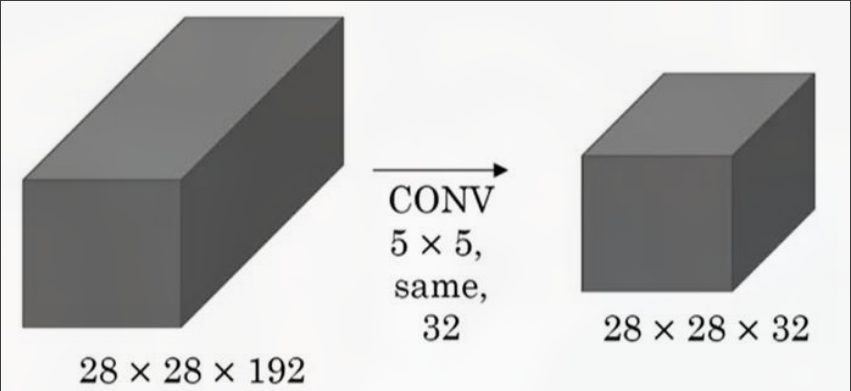
\includegraphics[width=\linewidth]{figures/big_vs_small_filters_1}
  Single big filter
\end{minipage}
\hfill
\begin{minipage}{0.58\textwidth}
  \centering
  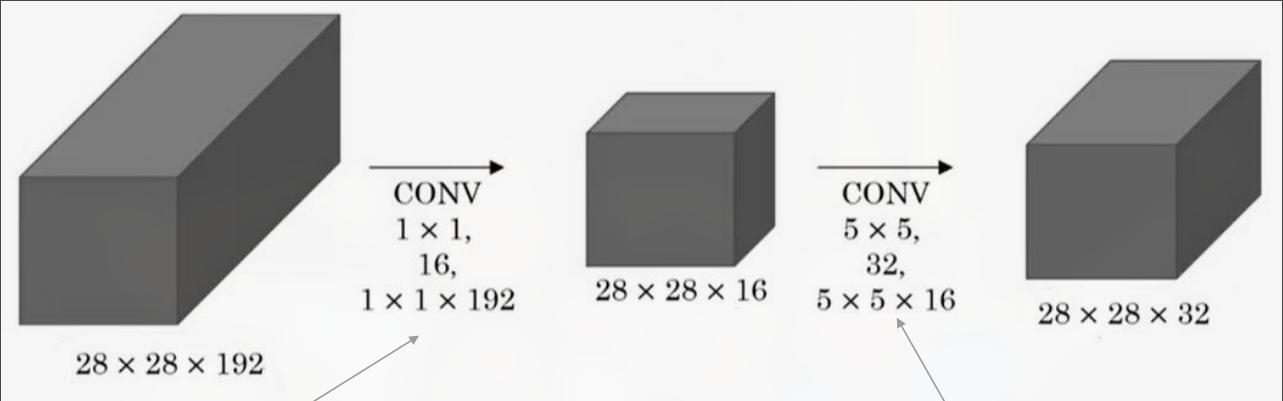
\includegraphics[width=\linewidth]{figures/big_vs_small_filters_2}
  Two smaller filters
\end{minipage}

\vspace{15pt}
The computational cost of the filter in the left picture is $28 \times 28 \cdot 5 \times 5 \cdot 32 \cdot 192 = 120$M, while the cost of the two smaller filters on the right picture is respectively $28 \times 28 \cdot 1 \times 1 \cdot 16 \cdot 192 = 2.4$M and $28 \times 28 \cdot 5 \times 5 \cdot 32 \cdot 16 = 10$M, so in total $ 2.4 + 10 = 12.4$M, which is circa 10 times less than using a single layer, but outputting the same result.

\newpage

\begin{note}
  The ``same'' value specified in the filter on the left image, means that the filter is padded with enough zeros to reach the same dimensionality of the input.
\end{note}

\begin{figure}[h]
  \centering
  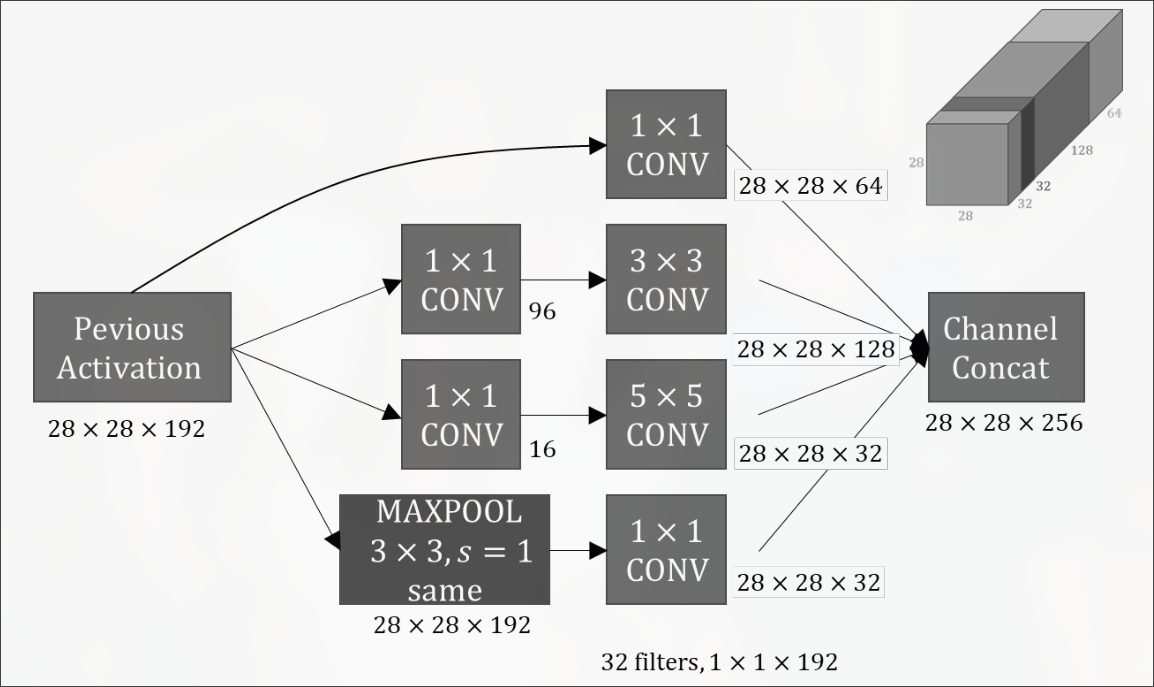
\includegraphics[width=0.55\linewidth]{figures/inception_module}
  \caption{Inception module developed by Google}
\end{figure}

\section{Localization and detection}

\textbf{Image classification}, classifies images based on the object it detects in them.
Exists also a variant \textbf{with localization} included, that after the detection, localizes the object by drawing a bounding box around it.
\textbf{Detection} differs from the previous two because is image classification with localization but for multiple objects (the previous models where single object detection).

In an object localization network, the output is split in two, on one branch there is a \textbf{softmax} function for the classification, while on the other there is a \textbf{regression} function that finds the coordinates of the object's bounding box.
Like we can see in the picture below, the output is split between a part for the classification and another for the bbox.

\begin{figure}[h]
  \centering
  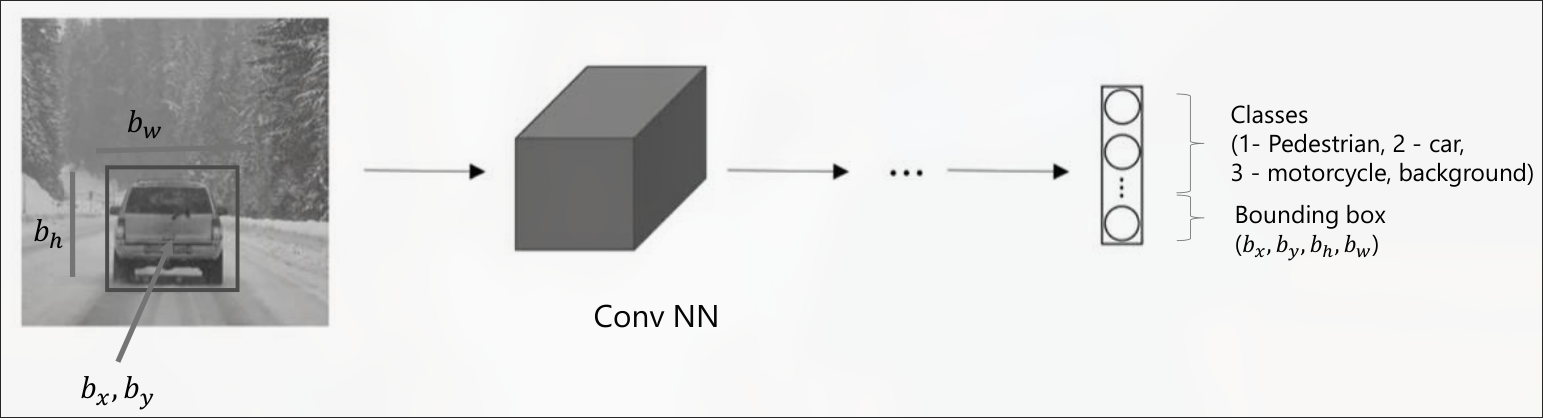
\includegraphics[width=0.8\linewidth]{figures/classification_with_localization}
\end{figure}

The \textbf{loss}, if there is an object in the image, takes care of all the output values, otherwise it takes care only of the $P_c$ value (the first one).

\newpage

\begin{figure}[h]
  \centering
  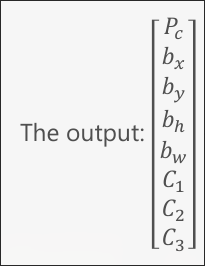
\includegraphics[width=0.17\linewidth]{figures/localization_output}
  \caption{Example of output vector}
\end{figure}

\textbf{Landmark detection}'s aim is to find specific points in an image, so is used, for example, in the recognition of people's faces or posture.

To be able to detect an object and also find its location, has been used the following idea: define a fixed size of the bounding box and use the box as a \textbf{sliding window} used to analyze only the portion of image isolated by the box and trying to detect any object inside.
This approach, however, is not robust in cases where the object can have \textbf{different scales}.
A possible patch to this problem is to scan multiple times the same image but with windows of different sizes or to \textbf{overlap} the boxes (usually is 50\% of the width).
\\\\
Using fully-connected layers, means that each pixel of the image influence every pixel in the following layer, while working with convolutional layers, if we select a specific portion of the image, then in the following layers, only a specific portion is strongly related to the previous portion and not the entire image.

Like we can see in the following figure, the top-left part of the image evidences the portions that are strongly related to each other, while proceeding in the network layers.

\begin{figure}[h]
  \centering
  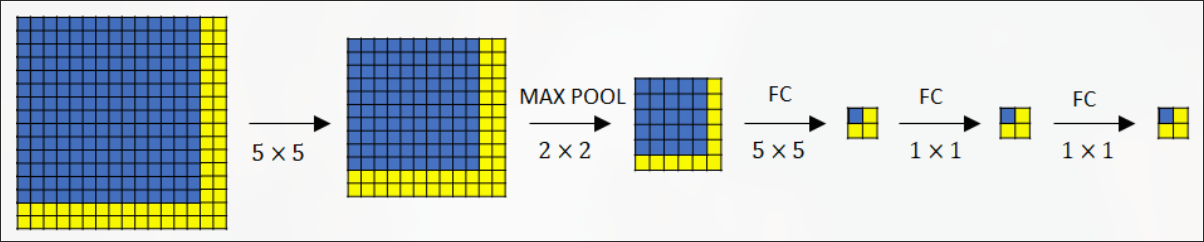
\includegraphics[width=0.8\linewidth]{figures/fc_vs_cnn}
\end{figure}

With fully-connected layers, we lose the spatial information.

Through the \textbf{spatial information} maintained by using convolutional layers, we're able to implement sliding windows, because we know that some specific points of the output depends on a specific (larger) portion of the input.
Using this strong relation is key to be able to use the sliding window approach.

\subsection{YOLO - You Only Look Once}

Using sliding windows led to another problem, which is that \textbf{not all} objects have a \textbf{square shape} (e.g. cars rectangular), so using square boxes give a not so accurate localization of them.
To solve this problem has been developed the YOLO algorithm, which is based on the following idea: using a \textbf{grid} over the image, where for each grid cell is associated a \textbf{vector} and each detected object is associated to only one cell (the location of the centroid object determines the associated grid cell).

\subsection{IoU - Intersection over Union}

To estimate the precision of the area of the predicted object location, is used the \textbf{Intersection over Union} approach, which is 
\begin{equation*}
  \text{Intersection over Union } = \frac{\text{area of intersection (overlap)}}{\text{area of union}}
\end{equation*}
This value returns the precision of the bbox respectively to the Ground-truth (the precise bbox annotation draw for the evaluation check).

\begin{figure}[h]
  \centering
  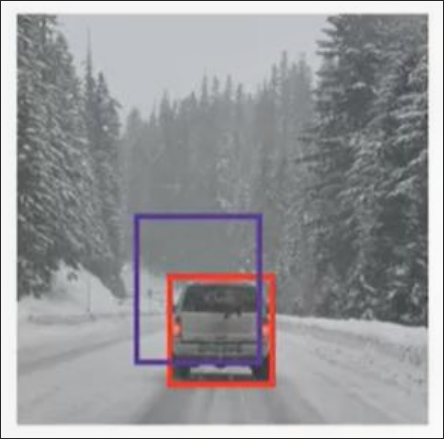
\includegraphics[width=0.25\linewidth]{figures/iou}
\end{figure}

In the figure above the blue (upper-left) box is the predicted bbox, while the other (the red down-right) is the Ground-truth one.
\\\\
Furthermore, can happen that we have multiple detections of the same object, so multiple bounding boxes.
To make the most precise deduction of the location is used the \textbf{Non-Max suppression} algorithm, which trivially discard all the detections that are not so secure.
This is achieved by fixing a lower bound for the $P_c$ value in the vector (e.g. $P_c > 0.6$, lower predictions are discarded).
If there are still multiple boxes, we pick the box with the largest $P_c$ output and then discard all the remaining boxes with IoU$ > 0.5$ against the picked box. 

With multiple-object detection, this process must be run for each object independently.

\section{Image Segmentation}

Can be split in two sub-categories:
\begin{itemize}
  \item \textbf{semantic} segmentation: find all the pixels that belong to a category (e.g. at a restaurant, detect the groups of people of the same table).
  \item \textbf{instance} segmentation: identify separately each single instance of a category (e.g. at a restaurant, detect each single person at the same table).
\end{itemize}

The architecture of image segmentation is based on two components (networks): an \textbf{encoder}, which extracts features by down-sampling the images (removes irrelevant details), and a \textbf{decoder} that takes in input the down-sampled images with only the important information and increases the dimension to reach back the original image size (up-samples the feature map).
\\\\
Among the scaling techniques there is the \textbf{up-sampling}, which scales up the image and is subdivided into two types:
\begin{itemize}
  \item nearest: copies the value from the nearest pixel.
  \item bilinear: linear interpolation from nearby pixels.
\end{itemize}

\chapter{RNN - Recurrent Neural Networks}\label{chapter:RNN}

The image below is a schema of a recurrent neural network:

\begin{figure}[h]
  \centering
  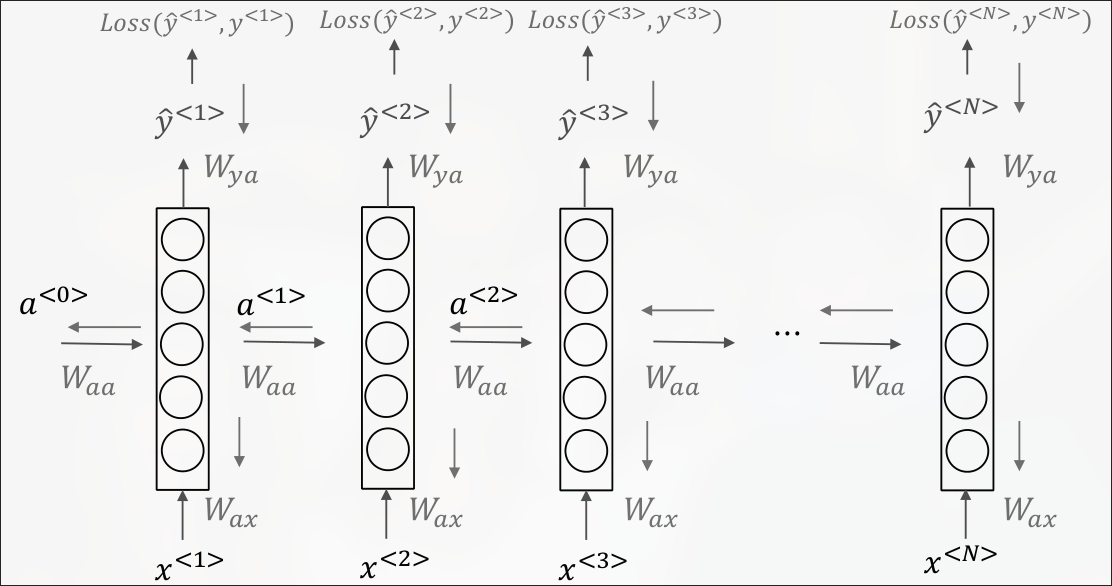
\includegraphics[width=0.6\linewidth]{figures/rnn}
\end{figure}

Each circle represents a \textbf{unit} (standard neural network with its own activation function), each rectangle is a hidden \textbf{layer}, $x$ is the \textbf{input} of the layer and is fully-connected to each hidden state (the units in the layer), $\hat{y}$ is the layer's \textbf{output} prediction (also the output is fully-connected with each hidden state) and $W$ are the \textbf{weights} that are shared.
The weights sharing properties makes our network suitable for variable-size inputs.
Hidden layers are fully-connected with their neighbor layers.

\textbf{Loss} simply calculates the loss between the prediction $\hat{y}$ and real output value $y$ and the backpropagation algorithm is called \textbf{Backpropagation Through Time} (BTT).

\begin{figure}[h]
  \centering
  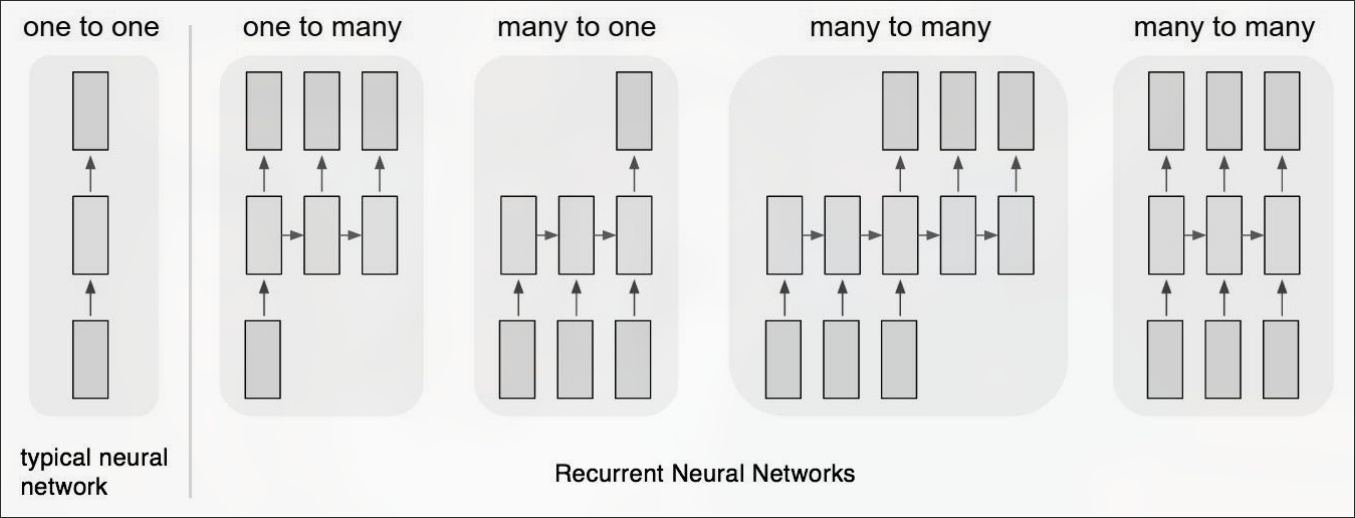
\includegraphics[width=0.7\linewidth]{figures/rnn_sequence_types}
\end{figure}

The above image, shows the different possible types of RNN sequences, where the bottom is the network input and the top is the network output.
\begin{itemize}[label=]
  \item \textbf{one to many} is used for image captioning, i.e. generates a sequence of words that represents the input image.
  \vspace{-8pt}
  \item \textbf{many to one} is mainly used for text classification (e.g. spam/not spam) or sentence correctness checking (e.g. verb time).
  \vspace{-8pt}
  \item \textbf{many to many} is commonly used for language translation (the input layers as a whole can be seen as a decoder, while the output layers as a single decoder), but also for automatic named entity extraction, depending on the configuration.
\end{itemize}

\newpage

\begin{figure}[h]
  \begin{minipage}{0.56\textwidth}
    \centering
    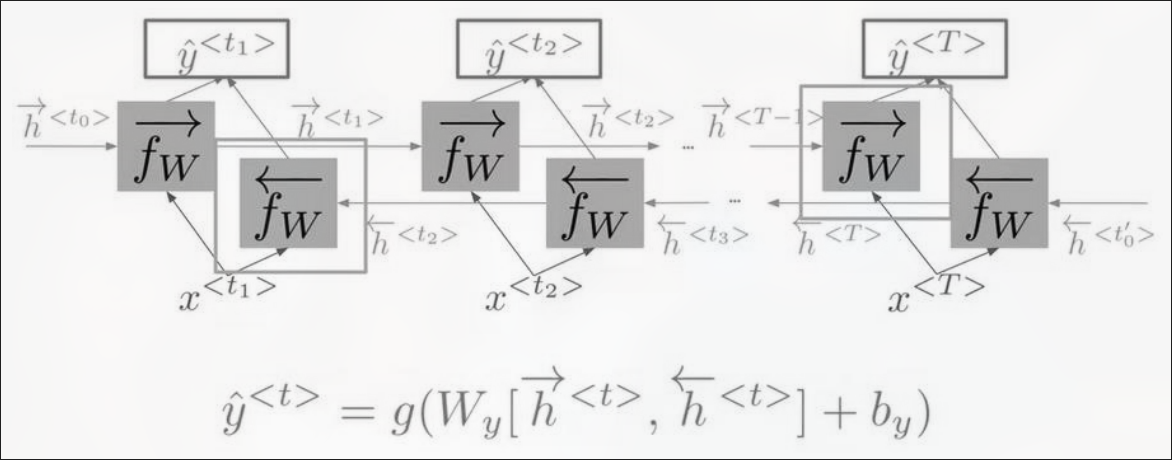
\includegraphics[width=\linewidth]{figures/bidirectional_rnn}
    \caption{Bidirectional RNN example}
  \end{minipage}
  \hfill
  \begin{minipage}{0.40\textwidth}
    \centering
    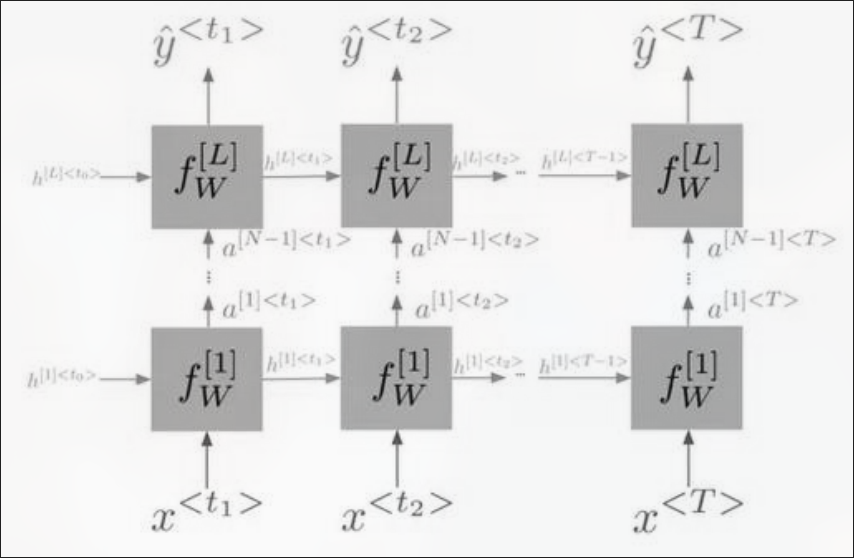
\includegraphics[width=0.85\linewidth]{figures/deep_rnn}
    \caption{Deep RNN example}
  \end{minipage}
\end{figure}

The equations of RNNs are (make reference to the first RNN image at the beginning of \textit{chapter~\ref{chapter:RNN}}):
\begin{align*}
  a^{\langle t \rangle} & = g_t \left( W_{aa} a^{\langle t-1 \rangle} + W_{ax} x^{\langle t \rangle} + b_a \right) = g_t\left( W_a \left[ a^{\langle t-1 \rangle}, x^{\langle t \rangle} \right] + b_a \right) \\
  \hat{y}^{\langle t \rangle} & = g^{\prime}_t \left( W_{ya} a^{\langle t \rangle} + b_y \right)
\end{align*}
where usually $g_t$ is a ReLU or a Tanh function and $g^{\prime}_t$ is a sigmoid function.
\\\\
Furthermore, we have that $W_a = \left[ W_{aa} W_{ax} \right]$ and $\left[ a^{\langle t-1 \rangle}, x^{\langle t \rangle} \right] = \begin{bmatrix} a^{\langle t-1 \rangle} \\ x^{\langle t \rangle} \end{bmatrix}$, in fact:
\begin{equation*}
  \left[ W_{aa} W_{ax} \right] \begin{bmatrix} a^{\langle t-1 \rangle} \\ x^{\langle t \rangle} \end{bmatrix} = W_{aa} a^{\langle t-1 \rangle} + W_{ax} x^{\langle t \rangle}
\end{equation*}

We introduced a new syntax for the formulas, because it represents better a state in a RNN in a more compact view, like in the image below:

\begin{figure}[h]
  \centering
  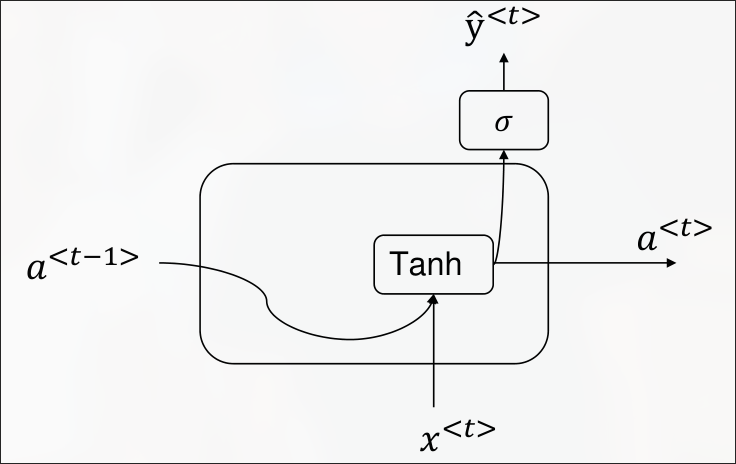
\includegraphics[width=0.4\linewidth]{figures/rnn_internal_state}
\end{figure}

\section{GRU - Gated Recurrent Unit}

An issue with the approach used also in the example at the beginning of \textit{chapter~\ref{chapter:RNN}}, is that we have different hidden states, one for each input, so researchers tried to find a more compact solution, that didn't require every time a new state for every input.
\textbf{Gated Recurrent Unit} is born as a solution for this problem, which is a particular hidden state because has an additional variable $c^{\langle t \rangle}$ (equal to $a^{\langle t \rangle}$ but present only in this unit) called \textbf{memory cell} and its job is to remember some important information relative to the time $t$.

\newpage

The \textbf{mechanism} of this unit for a specific time (step) $t$ in the network is:
\begin{enumerate}
  \item find a \textbf{candidate of} $\boldsymbol{c}$, which represents the hidden state $t$, and which formula is
    \begin{equation*}
      \tilde{c}^{\langle t \rangle} = \tanh \left( W_c \left[ c^{\langle t-1 \rangle}, x^{\langle t \rangle} \right] + b_c \right)
    \end{equation*}
  \item define a \textbf{gate} $\boldsymbol{u}$ s.t.
    \begin{equation*}
      \Gamma_u = \sigma \left( W_u \left[ c^{\langle t-1 \rangle}, x^{\langle t \rangle} \right] + b_u \right)
    \end{equation*}
    where $\Gamma_u \in \left\{ 0,1 \right\}$ and $u$ is referred as ``update''.
  \item lastly, \textbf{update} the value of $c$ using the formula
    \begin{equation*}
      c^{\langle t \rangle} = \Gamma_u \cdot \tilde{c}^{\langle t \rangle} + \left( 1 - \Gamma_u \right) \cdot c^{\langle t-1 \rangle}
    \end{equation*}
\end{enumerate}
\vspace{-20pt}
\begin{figure}[h]
  \centering
  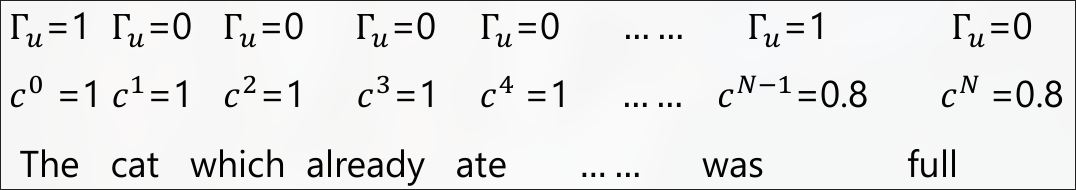
\includegraphics[width=0.6\linewidth]{figures/gate_example}
\end{figure}

As we can see in the example above, the value of the memory cell $c$ remain the same when the value of the gate $u$ is 0 and that's because in the updating formula 
\begin{align*}
  c^{\langle t \rangle} & = \Gamma_u \cdot \tilde{c}^{\langle t \rangle} + \left( 1 - \Gamma_u \right) \cdot c^{\langle t-1 \rangle} = \\
  & = 0 \cdot \tilde{c}^{\langle t \rangle} + \left( 1 - 0 \right) \cdot c^{\langle t-1 \rangle} = \\
  & = 0 + 1 \cdot c^{\langle t-1 \rangle} \\
  & = c^{\langle t-1 \rangle}
\end{align*}
the value of $c^{\langle t \rangle}$ is equal to the previous value $c^{\langle t-1 \rangle}$ if $\Gamma_u = 0$, but when instead is 1, the value of $c^{\langle t \rangle}$ is calculated like in a standard hidden state, because
\begin{align*}
  c^{\langle t \rangle} & = \Gamma_u \cdot \tilde{c}^{\langle t \rangle} + \left( 1 - \Gamma_u \right) \cdot c^{\langle t-1 \rangle} = \\
  & = 1 \cdot \tilde{c}^{\langle t \rangle} + \left( 1 - 1 \right) \cdot c^{\langle t-1 \rangle} = \\
  & = \tilde{c}^{\langle t \rangle} + 0 \cdot c^{\langle t-1 \rangle} \\
  & = \tilde{c}^{\langle t \rangle}
\end{align*}
and $\tilde{c}^{\langle t \rangle}$ formula is the same of $a^{\langle t \rangle}$ of a standard hidden state.
For this reason, like we can see in the picture, the value of $c^{\langle t \rangle}$ changes and the network knows that the previous cell was empty.

$c^{\langle t \rangle}$ behaves like a weighted combination of the previous states and the candidate state ($\tilde{c}^{\langle t \rangle}$).
\\\\
\begin{minipage}{0.38\textwidth}
  \centering
  GRU diagram:
\end{minipage}
\hfill
\begin{minipage}{0.60\textwidth}
  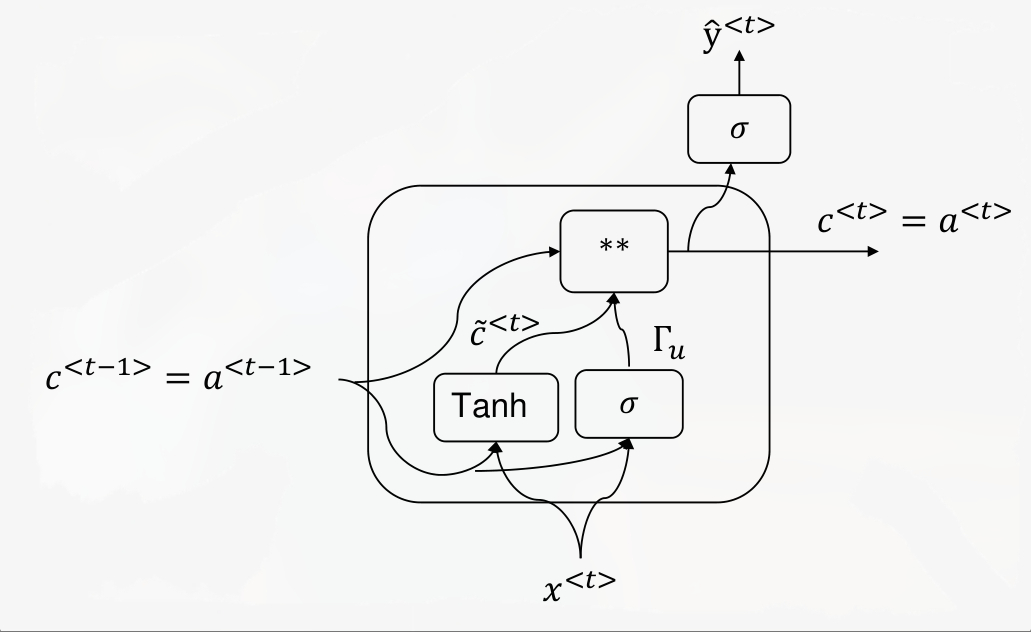
\includegraphics[width=0.7\linewidth]{figures/gru}
\end{minipage}

\newpage

The \textbf{Full GRU}, is a variant of the typical Gated Recurrent Unit just seen, in which is used an additional gate $r$ (stands for ``relevance''), which formula is
\begin{equation*}
  \Gamma_r = \sigma \left( W_r \left[ c^{\langle t-1 \rangle}, x^{\langle t \rangle} \right] + b_r \right)
\end{equation*}
and has been added by researchers, as a way to solve the vanishing gradient problem.

\section{LSTM - Long Short-Term Memory}

The formulas are:
\begin{flalign*}
  \qquad \tilde{c}^{\langle t \rangle} & = \tanh \left( W_c \left[ a^{\langle t-1 \rangle}, x^{\langle t \rangle} \right] + b_c \right) && \\
  \Gamma_u & = \sigma \left( W_u \left[ a^{\langle t-1 \rangle}, x^{\langle t \rangle} \right] + b_u \right) && \\
  \Gamma_f & = \sigma \left( W_f \left[ a^{\langle t-1 \rangle}, x^{\langle t \rangle} \right] + b_f \right) && \\
  \Gamma_o & = \sigma \left( W_o \left[ a^{\langle t-1 \rangle}, x^{\langle t \rangle} \right] + b_o \right) && \\
  c^{\langle t \rangle} & = \Gamma_u \cdot \tilde{c}^{\langle t \rangle} + \Gamma_f \cdot c^{\langle t-1 \rangle} && \\
  a^{\langle t \rangle} & = \Gamma_o \cdot c^{\langle t \rangle} &&
\end{flalign*}
where $\Gamma_u$ is the gate \textbf{update}, $\Gamma_f$ is the gate \textbf{forget} and $\Gamma_o$ is the gate \textbf{output}.

\begin{figure}[h]
  \centering
  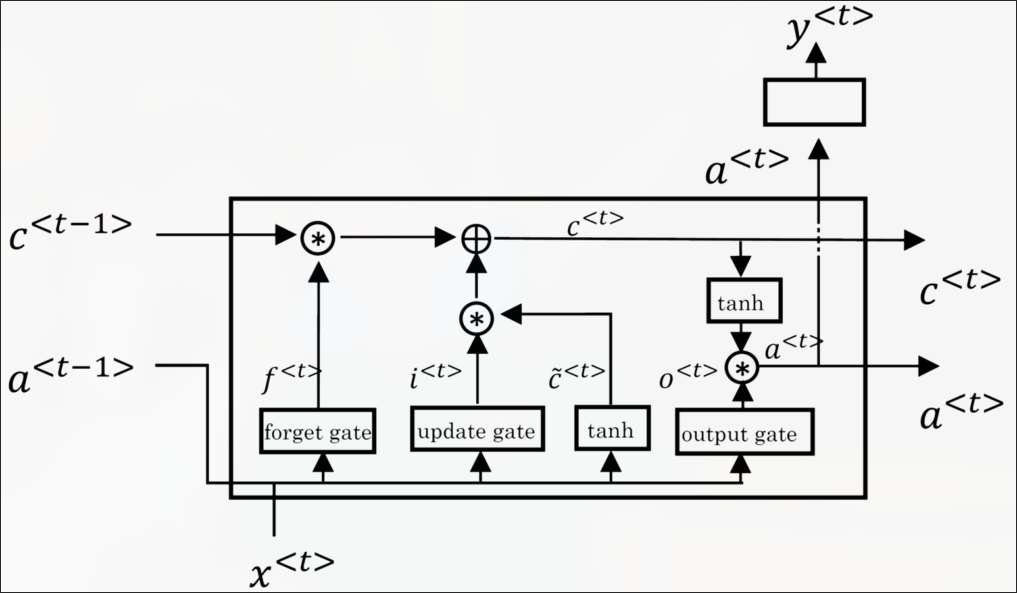
\includegraphics[width=0.5\linewidth]{figures/lstm}
  \caption{LSTM schema}
\end{figure}

If we train a LSTM with a vocabulary of 10000 words and 100-dimensional activations, the dimension of $\Gamma_u$ at each time step is 100.

\chapter{NLP - Natural Language Processing}

Possible applications areas are:
\begin{itemize}
  \item \textbf{Question answering}: receive a question, find the document more suitable for the question, extract the data and formulate an answer.
  \item \textbf{social media intelligence}: like sentiment analysis, so being able to identify what are the general emotions of the people about an action or a topic.
  \item \textbf{machine translation}: translate in real-time virtual communications (e.g. calls).
  \item \textbf{auto-responder}: reply to common messages or e-mails, identified through the matching over a template.
  \item \textbf{fake-news detection}: detect false information, by scanning text and confronting it with others, and also by checking the publisher and the author.
\end{itemize}

\section{Word Representation}

Word representation techniques represent words as feature vectors.
Combined with Deep Learning these techniques are state of the art in NLP in almost all the tasks. 
\vspace{5pt}

\begin{minipage}{0.48\textwidth}
  The simplest way to represent words as numbers is for a given vocabulary to assign a unique integer to each word, like in the image on the side.

  The set of unique words used in the text corpus is referred to as the \textbf{vocabulary}.

  This approach is simple, but has the \textbf{downside} of having an ordering with \textbf{little semantic sense}.
\end{minipage}
\hfill
\begin{minipage}{0.48\textwidth}
  \centering
  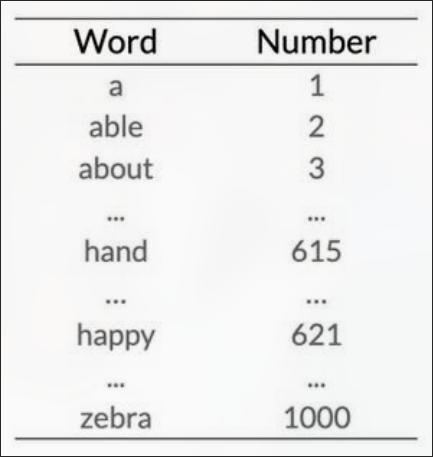
\includegraphics[width=0.52\linewidth]{figures/words_as_integers}
\end{minipage}

\vspace{5pt}
Another approach is called \textbf{one-hot vectors}, where each word in the vocabulary is mapped in a vector.
It's initialized with all 0's and to select a word we just set to 1 the value of the corresponding word, like in figure.
\vspace{-3pt}
\begin{figure}[h]
  \centering
  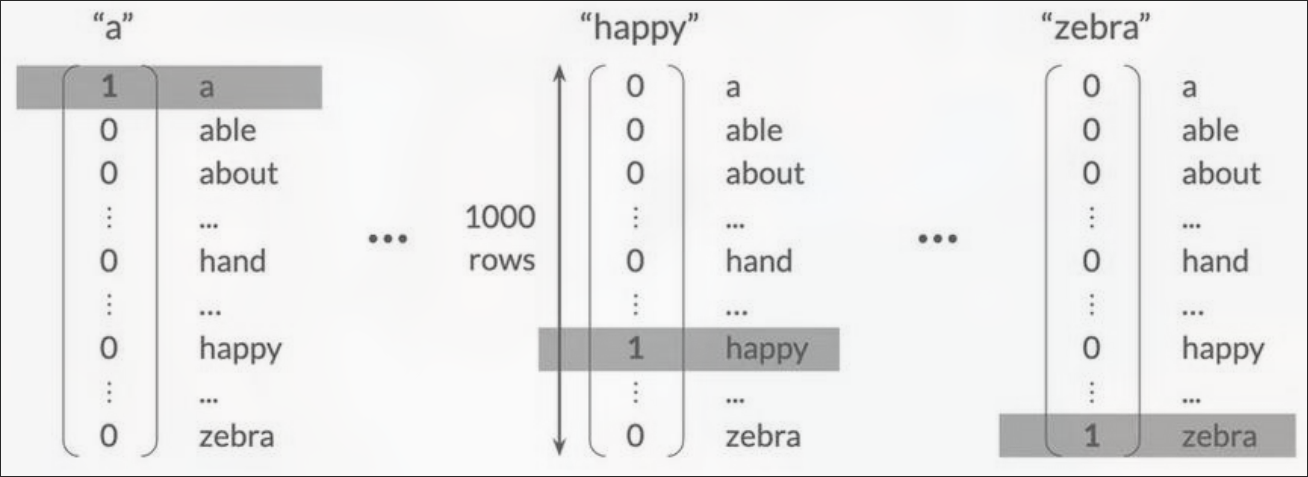
\includegraphics[width=0.6\linewidth]{figures/onehot_vector}
\end{figure}
\vspace{-3pt}

With this approach the ordering isn't needed, but arises new problems, like the \textbf{huge vector size} for big vocabularies and the \textbf{absence of an embedded meaning} in the structure.

\newpage

\textbf{Word embeddings} took the approach of one-hot vectors, but fixed the embedded meaning problems, in fact are vectors which also carry the meaning.
Words are mapped in the vector, like they're placed over the x-axis, because more a word is on the left (at the beginning of the vector), more has a ``negative'' meaning, while on the opposite, on the farthest right are placed the ``positive'' words.
For this reason ``negative'' words have a negative value, while ``positive'' words have a positive one and the closer is a word to the middle (the 0 of the x-axis), more neutral is their meaning.

\begin{figure}[h]
  \centering
  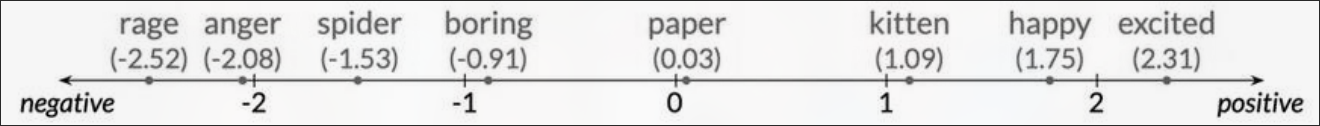
\includegraphics[width=0.7\linewidth]{figures/word_embedding}
\end{figure}

Researchers extended this approach by adding also a y-axis, associated with the level of concreteness (positive for ``concrete'', negative for ``abstract''), like in the figure:

\begin{figure}[h]
  \centering
  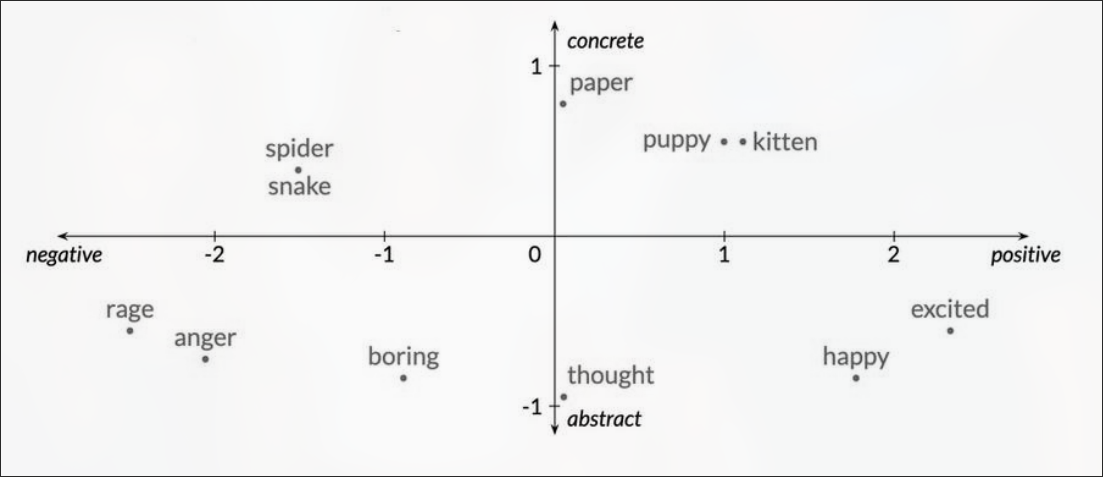
\includegraphics[width=0.65\linewidth]{figures/word_embedding_extended}
\end{figure}

We can also increase the dimensionality over 2, adding more layers, but this will increase the difficulty of choosing a value for each word.

This final approach has an embedded meaning, because it orders word while creating a semantic distance and all while keeping a low dimensionality.
\\\\
If we wanted to capture the full range of variation and meaning over our vocabulary of size $n$, also the word embeddings vector should have a size of $n$ (e.g. 1000 words, 1000 embeddings).

\begin{figure}[h]
  \centering
  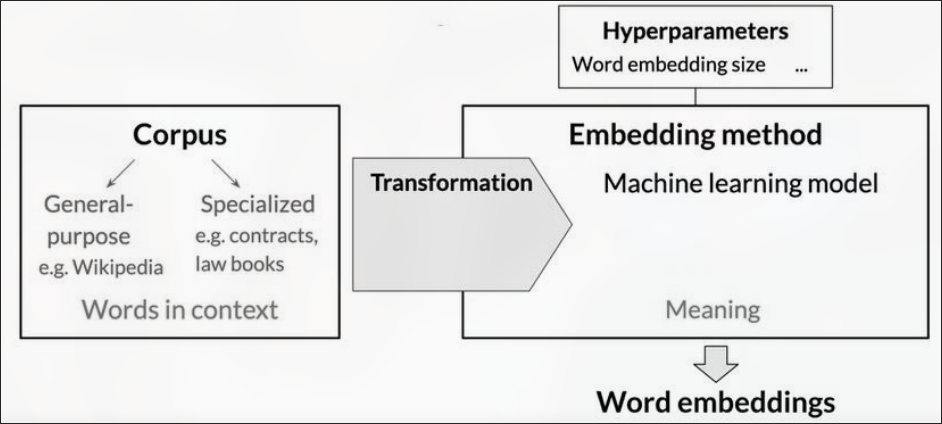
\includegraphics[width=0.55\linewidth]{figures/word_embedding_schema}
\end{figure}

The figure above is the schema of the word embedding process:
\begin{enumerate}
  \item inputs are the text corpus and some hyperparameters, like the word embedding size (usually 300/500).
  \item through a machine learning model, words are arranged with the \textbf{embedding method}.
  \item lastly, are outputted all the word embeddings, which is a set of numbers (points in our feature space).
\end{enumerate}

\section{Word2Vec}

\textbf{Word2Vec} network is a technique for building a rich semantic word embedding space and implements the idea that two words have similar word embedding representations if they have similar contexts.

This network is born as a solution for the following problem: 
\begin{quote}
  \textit{given a vocabulary and an input word, what are the probabilities of each vocabulary word that, in a possible sentence, is ``near'' to the input word?}
\end{quote}
where ``near'' is represented using a sliding window and its size corresponds to the number of words that precede or follow the input word.
Usually the size is 5 and this means that the network will look for 5 words behind and 5 words ahead of the input word.
\\\\
To train the network and create a dataset, the researchers made the opposite: from a sentence they used the sliding windows, to generate all the tuples of the type \textit{(input\_word, near\_word)}, like in the figure below (example with window size 2):

\begin{figure}[h]
  \centering
  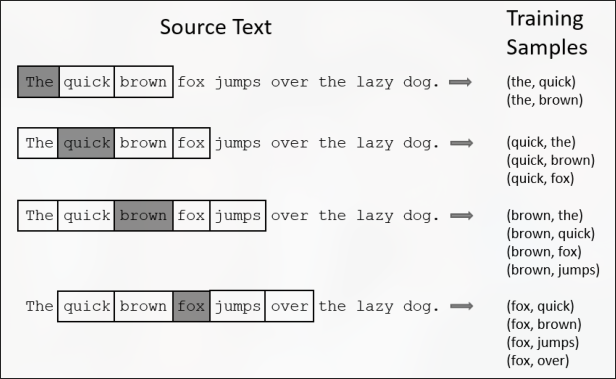
\includegraphics[width=0.6\linewidth]{figures/word2vec_training}
\end{figure}

The network trained on this sentence, if tested with the word ``quick'' should return high probabilities for the words ``the'', ``brown'' and ``fox'' and values as low as possible for the other words.
The network is going to learn the statistics from the number of times each pairing shows up.

\begin{figure}[h]
  \centering
  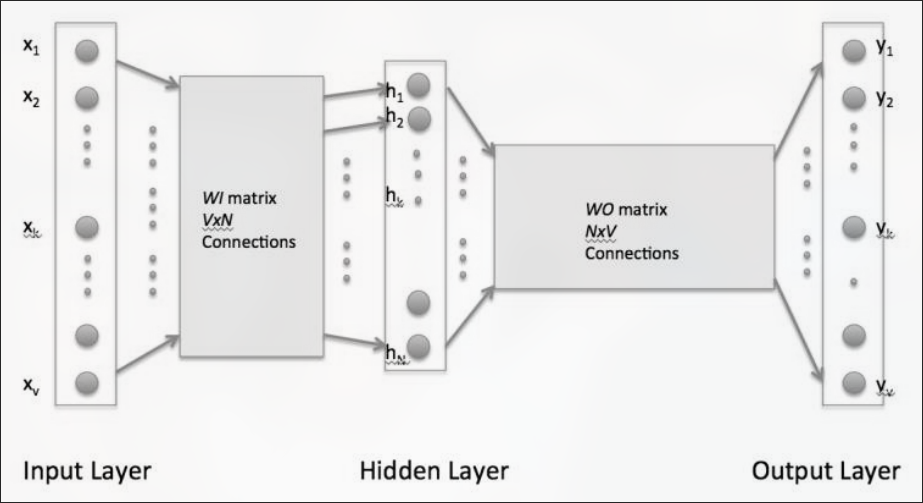
\includegraphics[width=0.6\linewidth]{figures/word2vec_model}
  \caption{Word2Vec network model}\label{fig:word2vec_model}
\end{figure}

The network, schematized in the Figure~\ref{fig:word2vec_model}, is composed only of an input layer, an intermediate hidden layer and an output layer.
Both \textbf{input} and \textbf{output} have the \textbf{same size}, because in output we have the vocabulary, where each word is paired with a probability, and in input we have a one-hot vector with the words, so has the same size of the vocabulary and is set to 1 only in the position of the input word.
In the hidden layer, the number of features usually is around 300, so the weight matrix that represents the hidden layer will be $\textit{vocabulary\_size} \times 300$.
This network particularity is that has \textbf{no activation function} on the hidden layer neurons, while in the output layer is applied a \textbf{softmax function}, in order to obtain probabilities in the range [0,1].
\\\\
In real vocabularies, frequent words like conjunctions, pronouns, ecc (e.g. ``the'') are not present and also all those words that always come together (e.g. ``New'' ``York''), are treated as a single word.

\section{Transformers}

\textbf{BERT} (Bidirectional Encoder Representations from Transformers) is a paper published by researchers at Google AI Language.
BERT’s key technical innovation is applying the \textbf{bidirectional training} of Transformer, a popular attention model, \textbf{to language modelling}.
In short BERT consists of only the \textbf{Encoder} part of the Transformer introduced in the paper ``Attention Is All You Need'', with some novel modifications. 
\\\\
Transformer was developed for solving text translation problem and its architecture consists of an \textbf{encoder} and a \textbf{decoder}, where the encoder’s output is given as input to the decoder.

\begin{figure}[h]
  \centering
  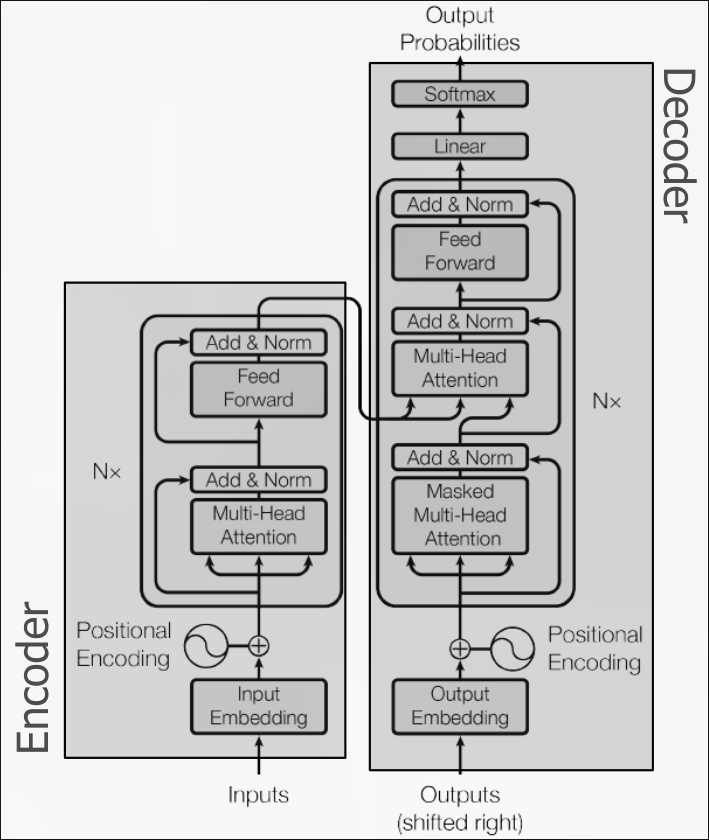
\includegraphics[width=0.4\linewidth]{figures/transformer}
  \caption{Transformer ``Attention is all you need''}\label{fig:transformer}
\end{figure}

\newpage

\subsection{Encoder}

The input is a sequence of tokens, which are first embedded into vectors and then processed in the neural network.
The output is a sequence of vectors of size H, in which each vector corresponds to an input token with the same index.

\begin{figure}[h]
  \centering
  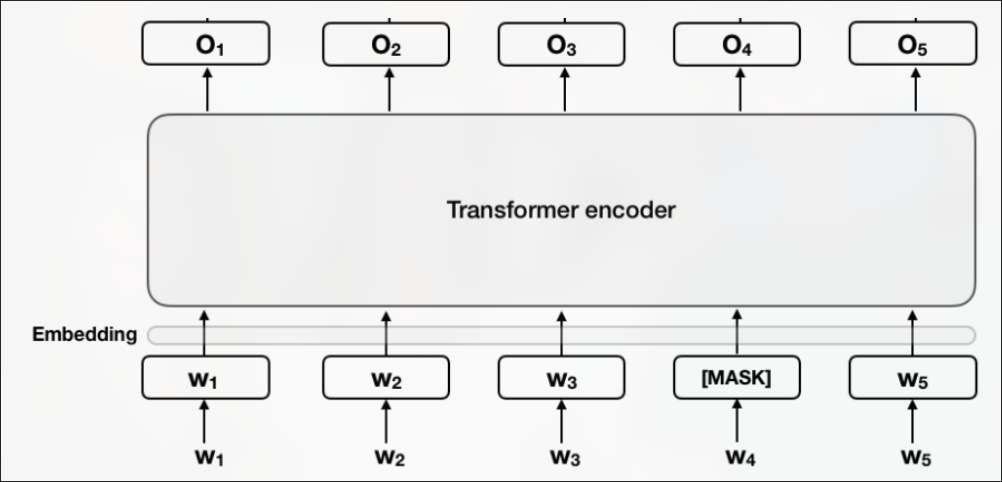
\includegraphics[width=0.6\linewidth]{figures/transformer_encoder}
\end{figure}

Because the size doesn't change, we can stack multiple encoders creating the so-called \textbf{information flow}.
The architecture is the following:
\begin{enumerate}
  \item The model represents each token as a vector of \textit{embedded\_dimension} size. We have a matrix of dimension $\textit{input\_length} \times \textit{embedded\_dimension}$ for a specific input sequence (sentence). The \textit{input\_length} corresponds to the number of words.
  \item Is added positional information to each token, called \textbf{positional encoding}, which, at the beginning of the training, are initialized with random numbers. The matrix size remains the same.
  \item The data goes through N encoder blocks. After this, we obtain the same matrix dimension.
\end{enumerate}
\vspace{-10pt}
\begin{figure}[h]
  \centering
  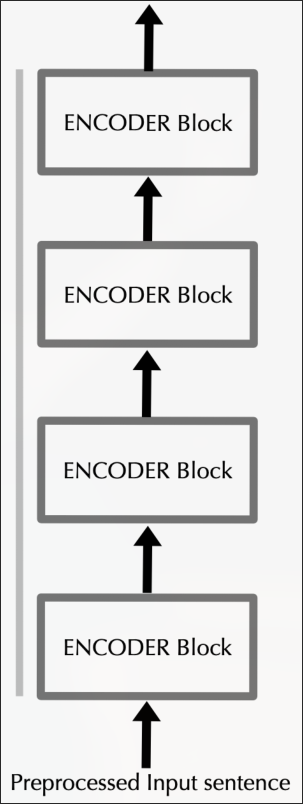
\includegraphics[width=0.2\linewidth]{figures/information_flow}
  \caption{example with $\text{N}=4$}
\end{figure}

Points 1 and 2 are done during the \textbf{input preprocessing}.
The blocks do not share weights.

\newpage

The transformation from words to vectors is done like in RNNs and the steps are:
\begin{enumerate}
  \item \textbf{tokenization}: split the words and also punctuation (\textit{e.g.} ``?'' is important for the phase structure and meaning) in the sentence.
  \item \textbf{numericalization}: process of mapping each token to a unique integer in the vocabulary.
  \item \textbf{word embeddings}: each word is mapped to a vector of size \textit{embedded\_dimension} that the model will learn during the training and the elements of those vectors are treated as model parameters and are optimized with back-propagation just like any other weights.
\end{enumerate}

The \textbf{padding} is added to the input sequences in order to keep the \textbf{same size} for each batch.
\\\\
Each \textbf{block} in the encoder is in charge of \textbf{finding relationships} between the input representations and encode them in its output.
This \textbf{iterative process} through the blocks guarantees that the neural network \textbf{captures complex relationships} between words.

\subsection{Multi-Head Attention}

The transformer uses \textbf{multi-head attention} and this means that it computes the attention \textbf{multiple times with different weights} and then concatenates the results together.

\begin{figure}[h]
  \centering
  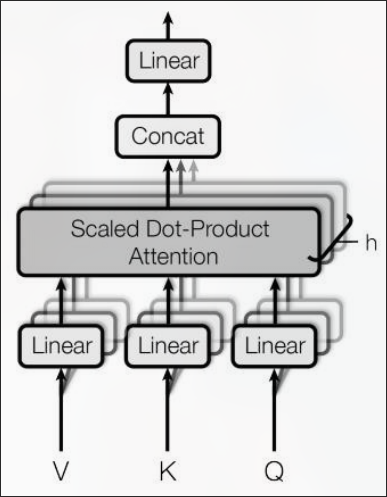
\includegraphics[width=0.3\linewidth]{figures/multihead_attention}
  \caption{multi-head attention schema}
\end{figure}

In the figure above is represented the multi-head attention mechanism, which takes in input multiple matrices of the same size (\textit{e.g.} $516 \times 300$) that are processed in parallel through linear functions (attention functions), which result is merged into one single output called \textbf{head} and used in the \textbf{scaled dot-product attention}.
That's the origin of this process' name, in fact we have the concatenation of multiple heads (in the image there is a total of $h$ heads) produced by the attention functions.

The formula is:
\begin{equation*}
  \text{MultiHead}(Q,K,V) = \text{Concat}(\text{head}_1, \text{head}_2, \ldots, \text{head}_h) \cdot W^O
\end{equation*}
where $\text{head}_i = \text{Attention}(QW_i^Q, KW_i^K, VW_i^V)$.

\newpage

Let's rename the following products as $QW_i^Q = Q_i$, $KW_i^K = K_i$ and $VW_i^V = V_i$, then the Attention's formulas is:
\begin{equation*}
  \text{Attention}(Q_i, K_i, V_i) = \text{Softmax} \left( \frac{Q_i \cdot K_i^T}{\sqrt{d_k}} \right) \cdot V_i
\end{equation*}

Remember $Q_i$ and $K_i$ are different projections of the tokens into another dimensional space ($d_k$).
Therefore, we can think about the dot product of those projections as a \textbf{measure of similarity} between tokens projections.

If we call $v_i$ and $u_j$ the projections of the i-th token and the j-th token through $Q_i$ and $K_i$ respectively, their dot product can be seen as:
\begin{equation*}
  v_i u_j = \cos \left( v_i, u_j \right) \lVert v_i \rVert_2 \lVert u_j \rVert_2
\end{equation*}
where $\lVert v_i \rVert_2$ is the normalization of the vector $v_i$.

This product measures how similar are the \textbf{directions} of $v_i$ and $u_j$, and how large are their \textbf{lengths} (the closest the direction and the larger the length, the greater the dot product).
\\\\
The network will learn through the training process which \textbf{relationships} are more useful and will relate tokens to each other, based on these relationships.
We can think about the resulting representation of word as a weighted combination (centroid) of the projected vectors through $V_i$ of the input tokens.
\\\\
The \textbf{position-wise feed-forward} component (that we can see in Figure~\ref{fig:transformer}) just takes a fully-connected linear layer and applies a ReLU to it.
\\\\
The \textbf{add \& norm} component applies a dropout at $10 \%$ in the input and the result is added to the original input.
It's used to keep the information already learned while also learning new relationships with the remaining tokens.

\subsection{Training}

When training language models, there is a challenge of defining a \textbf{prediction goal}.
Many models predict the next word in a sequence, but it's a directional approach which inherently \textbf{limits context learning}.
To overcome this challenge, BERT uses two training strategies simultaneously: \textbf{Masked Language Model} and \textbf{Next Sentence Prediction}.

\paragraph{Masked Language Model}

Given a sequence of words, one word is masked and then the sequence is given in input to the model.
Then, if the model predicts correctly the word ID, the weights remain the same, otherwise, the weights are updated, \textit{i.e.} the embedding value of the masked word in the dictionary is replaced with the embedding output of the model for the masked word.
Before feeding word sequences into BERT, $15\%$ of the words in each sequence are replaced with a [\textit{MASK}] token.

\paragraph{Next Sentence Prediction}

Find if two or more sentences that compose the sequence of words makes sense or not, \textit{i.e.} a sentence is the following of the previous one. There is no human interaction or preparation, we can just automate all the process by randomly selecting the masked word and the sentences sequence, from pieces of given piece of text.

\subsection{Fine-Tuning}

At the end of the training we obtain a pre-trained BERT model, that can be used for a wide variety of language tasks, by only adding some small layers to the core model and this is called \textbf{fine-tuning}.
This process differs based on the final task we need for the model:
\begin{itemize}
  \item \textbf{Classification} - given in input a sentence to a model (encoder or decoder), it outputs a classifier; a set with the probabilities of belonging to a specific class in the set.
  \item \textbf{Question Answering} - given in input a question and a text related to the question, the model through a regression should be able to compose an answer using the information extracted from the text (\textit{.i.e.} returns the position of the answer in the text)
  \item \textbf{Named Entity Extraction} - given a text, the model should be able to classify each word in a specific class (entity).
  \item \textbf{Named Entity Recognition} - is similar to the previous, with the difference that instead of finding the entities for the text, it recognizes the words that belong to specific entities.
\end{itemize}

\subsection{Decoder}

Has similar components to the encoder, except for a \textbf{Masked Multi-Head Attention} component.

\section{GPT}

Instead of using the encoder, for the GPT they used the \textbf{decoder}.
GPT differentiate from BERT because, given an input text, it tries to answer by finding each time the \textbf{most correct word that follows} the preceding ones in the sentence.
That's the reason why using a GPT we have an answer composing animation.

\subsection{Masked Self-Attention}

\begin{figure}[h]
  \centering
  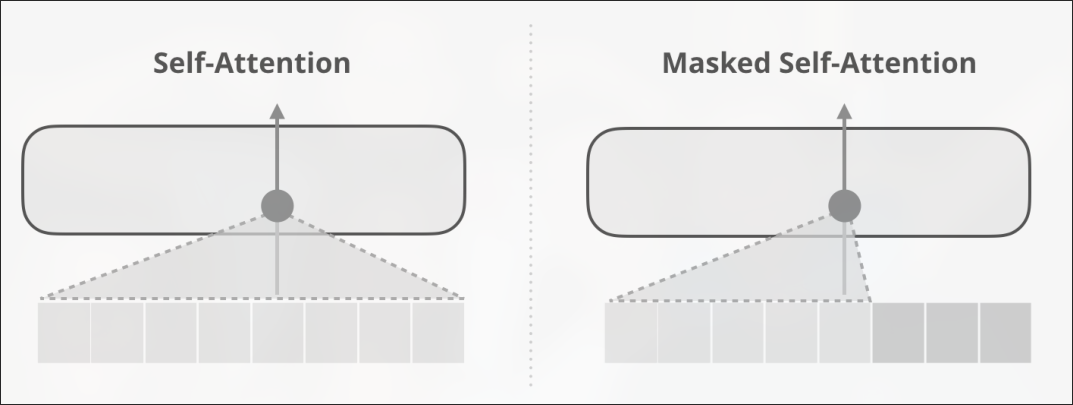
\includegraphics[width=0.6\linewidth]{figures/masked_selfattention}
  \caption{Plain vs. Masked self-attention}\label{fig:masked_selfattention}
\end{figure}

Every time we want to predict a new word based on what we saw before.
This is crucial because in a GPT model we can't use future information (\textit{i.e.} the following words).
This component implements a mask that shows only words until a certain point and the following are hidden, like in Figure~\ref{fig:masked_selfattention}.

\subsection{ChatGPT}

Has been developed following this growth steps:
\begin{enumerate}
  \item Language Model (Self-Supervised Learning)
  \item Question Answering (Supervised Learning)
  \item Reinforcement Learning from Human Feedback (RLHF)
\end{enumerate}

As a final development step, the researchers engineered a prompt in a way that the model could interpret correctly the input:
\begin{itemize}
  \item writing clear and specific instructions, using delimiters (like `', ``'', $<>$, etc.).
\end{itemize}

\chapter{GNN - Graph Neural Networks}

Are used for representing:
\begin{itemize}
  \item \textbf{molecules}
  \item \textbf{images}: graphs with regular structure (e.g. squared) where each node represents a pixel of the image and is connected with the adjacent nodes. Each single node is a 3-dimensional vector representing the RGB value.
  \item \textbf{text}: by indexing each character or word into a node, we can represent sentences as a sequence of nodes through a Direct Acyclic Graph, where words are connected with edges.
  \item \textbf{social networks}: each people/group of people is represented as a node and the relationships are the edges.
\end{itemize}

\section{Predictions on graphs}

\begin{itemize}
  \item \textbf{graph-level} task: predict the property of an entire graph, e.g. detect the nodes with 2 rings (Figure~\ref{fig:two_rings_example})
  \item \textbf{node-level} task: concerned with predicting the identity or role of each node within a graph (e.g. Zach’s karate club: club schism, find which members (nodes) followed the first instructor and those that followed the other, \textit{i.e.} identify the split of the nodes in the graph).
  \item \textbf{edge-level} task: used for example in image inferring for film scene understanding, \textit{i.e.} detect objects or people and identify their current action.
\end{itemize}

\begin{figure}[h]
  \centering
  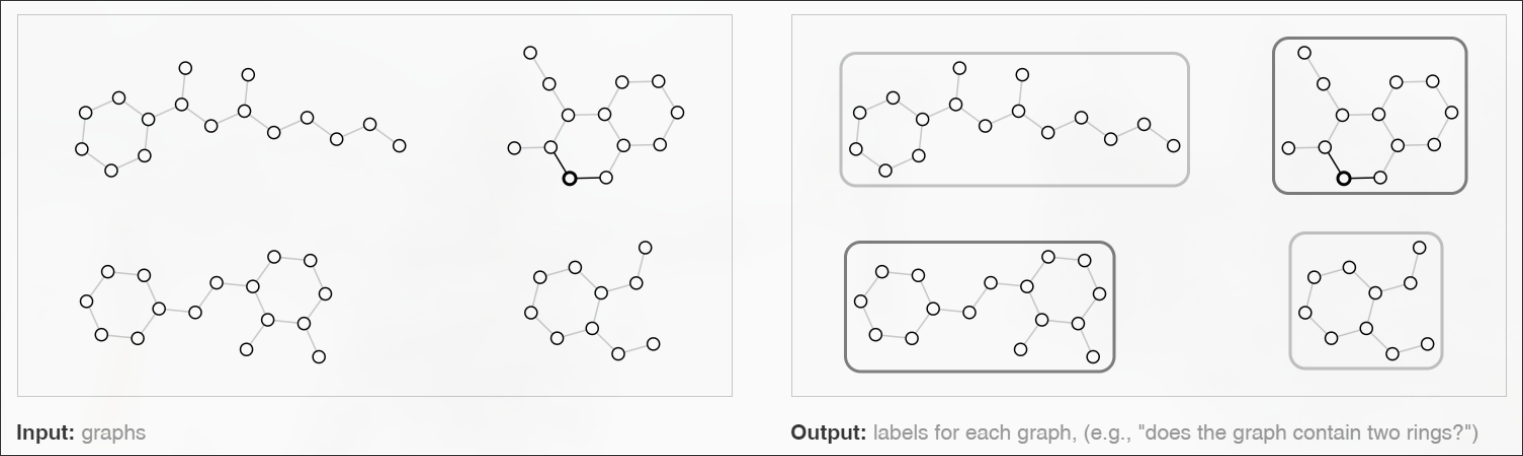
\includegraphics[width=0.7\linewidth]{figures/two_rings_example}
  \caption{Example of graph-level task}\label{fig:two_rings_example}
\end{figure}

\newpage

\section{GNN Models}

GNN's adopt a ``graph-in, graph-out'' architecture, meaning that these model types accept a graph as input and progressively transform these embeddings, without changing the connectivity of the input graph.
As is common with neural networks modules or layers, we can stack these GNN layers together.

\begin{figure}[h]
  \centering
  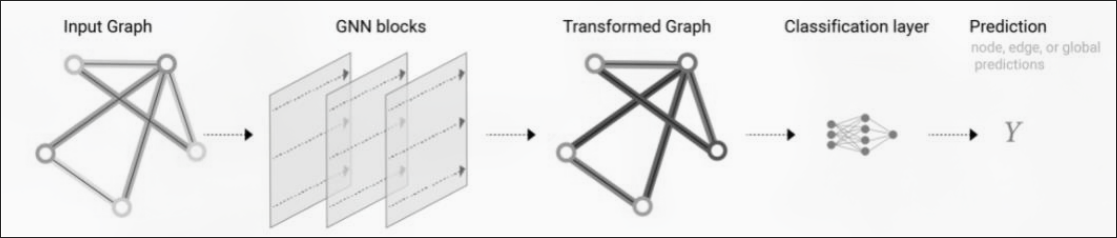
\includegraphics[width=0.7\linewidth]{figures/gnn_example}
  \caption{End-to-end prediction task with a GNN model}
\end{figure}

In the block the GNN uses a separate multilayer perceptron (MLP) on \textbf{each component} of the graph.
Thus for each node and edge the \textbf{MLP} is applied and we obtain the learned \textbf{embeddings} for each of those, that in the overall make up the transformed graph.

Now, we can make predictions \textbf{over the transformed graph} that has been outputted and the approach is straightforward: for each node embedding, we \textbf{apply a linear classifier}.
\\\\
However, it is not always so simple because, for example, we might have information about the graph only stored in the edges and none in the nodes, but we still need to make predictions on nodes.
A solution is to \textbf{pool} information from the edges and give it to the nodes and this happens in two steps:
\begin{enumerate}
  \item For each item to be pooled, we \textbf{gather} each of their embeddings (vector) \textbf{and concatenate} them (matrix).
  \item The gathered embeddings are \textbf{then aggregated}, usually via a sum or mean operation, \textit{i.e.} each line of the matrix becomes a single cell, thus the matrix becomes a vertical vector.
\end{enumerate}
The pooling operation is represented with the symbol $\rho$ (rho) and the pooling from edges to nodes $\rho_{E_n \rightarrow V_n}$.

\section{Message Passing}

Until now, we were \textbf{not using the connectivity} of the graph, instead we were using the information of each component independently.
Instead, we could make \textbf{more sophisticated predictions} by using pooling within the GNN layer, in order to make our learned embeddings aware of graph connectivity.
We can achieve this by using \textbf{message passing}, where neighbor nodes or edges exchange information and influence each other on their updated embeddings.
This technique is split in three steps:
\begin{enumerate}
  \item gather all the neighbors' node embeddings (or messages)
  \item aggregate all messages (e.g. sum)
  \item pass all through an update function, usually a learned neural network
\end{enumerate}
Message passing can occur between either nodes or edges indifferently.

\newpage

\begin{figure}[h]
  \centering
  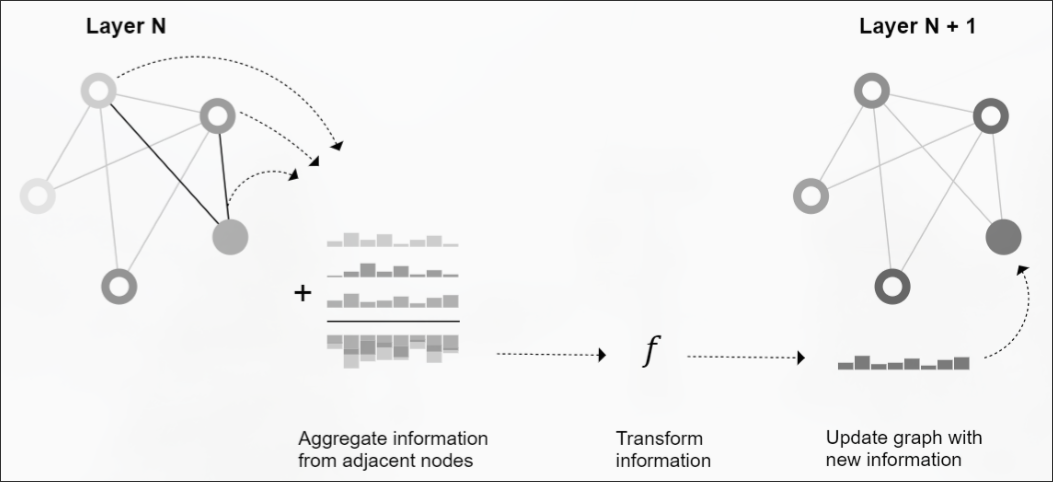
\includegraphics[width=0.7\linewidth]{figures/message_passing}
  \caption{Example of Message Passing over the full node in the image}
\end{figure}

The difference with the previous and easier approach is that to the transformation function are given in input multiple information (the one of the node plus those of the adjacent nodes), while before we only gave the nodes' one.
\\\\
In essence, Message Passing is similar to Convolution because are operations that aggregates and process information of an element’s neighbors in order to update the element’s value.
In graphs, the element is a node, while in images, the element is a pixel and this makes some difference because in images each pixel has a fixed number of neighbors, while in graphs this number is variable.
However, with graphs, we're able to pass multiple GNN layers together, so a node can incorporate information from the entire graph, e.g. after three layers, a node has information about the nodes three steps away from it.

\chapter{Optimization}

\section{Batch vs. Mini-Batch Gradient Descent}

When you are using the Gradient Descent is used the entire training set to compute the Cost function and the derivatives.
However, it’s prohibitive when you are dealing with very large-scale datasets.
For this reason we can split the dataset into smaller mini-batches which the Gradient will compute one at a time separately.
This strategy is obviously called \textbf{Mini-Batch Gradient}.

\begin{figure}[h]
  \centering
  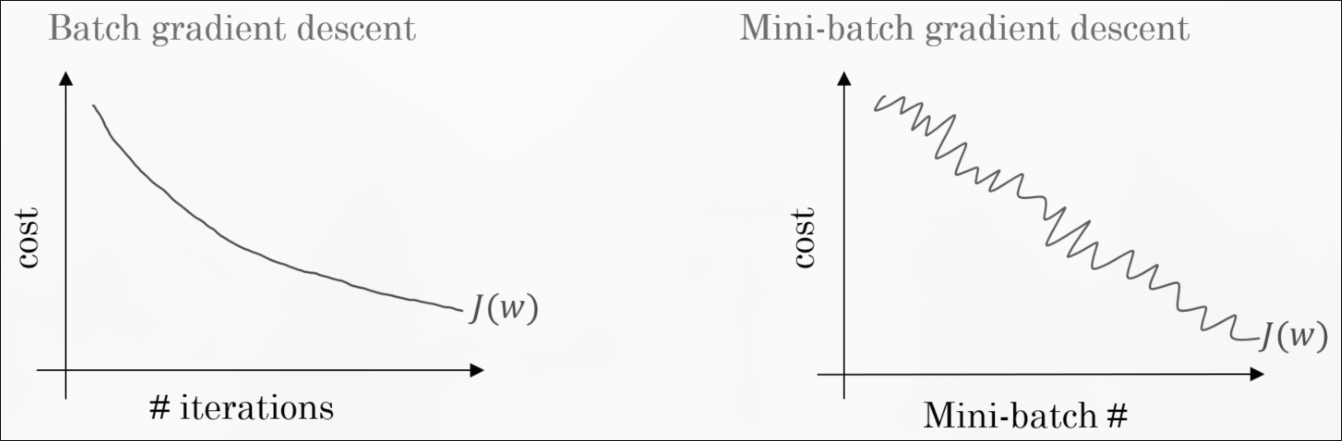
\includegraphics[width=0.6\linewidth]{figures/mini_batch_graph}
\end{figure}

As we can see in the figure above, the mini-batch gradient curve isn't smooth as the single-batch because we can have mini-batches that are more difficult than others.
\\\\
To the opposite side of the Batch Gradient Descent approach there is the \textbf{Stochastic Gradient Descent}, which works over batches of size 1, so obviously doesn't use vectorization because takes one element at a time, but it's really slow.
Normal Batch Gradient Descent takes the maximum size $m$ of the input dataset and uses it all, thus requiring a huge memory space for vectorization.
Mini-Batch Gradient Descent is the intermediate solution between these two extremes.
\\\\
If we have a small training set, like 2000 samples, we can just use Batch Gradient Descent, while, if we have a larger training set, the typical mini-batch sizes are 64, 128, 256, 512 and 1024.

\section{Algorithms}

\subsection{Exponentially weighted average}
\begin{equation*}
  V_t = \beta V_{t-1} + (1-\beta) \theta_t
\end{equation*}
where $V_t$ is the weighted average value at time $t$, $\beta$ is the weight factor and $\theta$ is the recorded value at time $t$.

\newpage

Because this formula doesn't return good result with low value for $t$, we can use \textbf{bias correction} to adjust the value and the formula is:
\begin{equation*}
  \tilde{V}_t = \frac{V_t}{1-\beta^t}
\end{equation*}
where $\tilde{V}_t$ is the corrected $V_t$ value.

\subsection{Gradient Descent with Momentum}

Almost always works empirically faster than standard gradient descent algorithm.
For each iteration compute $\diff{\mathcal{L}}{W}$ and $\diff{\mathcal{L}}{b}$ and the new values of $dW$ and $db$ are
\begin{align*}
  & V_{dW} = \beta V_{dW} + (1-\beta) \diff{\mathcal{L}}{W} \\
  & V_{db} = \beta V_{db} + (1-\beta) \diff{\mathcal{L}}{b}
\end{align*}
where a good value for $\beta$ is $0.9$ and the final updated values for $W$ and $b$ are:
\begin{align*}
  & W = W - \alpha V_{dW} \\
  & b = b - \alpha V_{db}
\end{align*}

\begin{figure}[h]
  \centering
  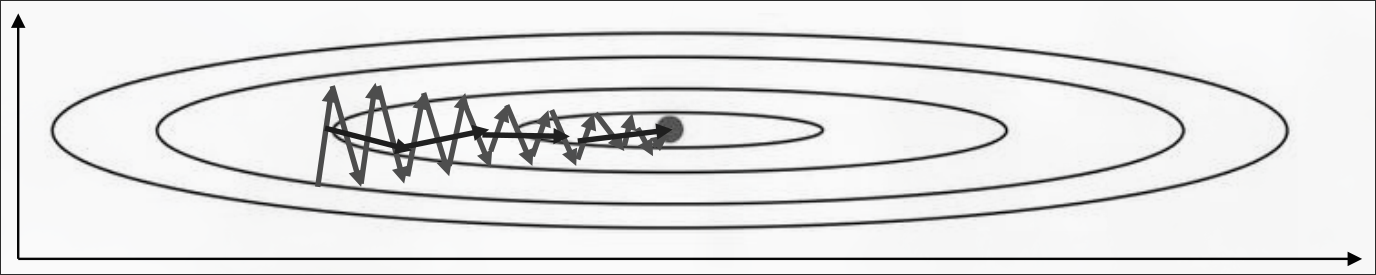
\includegraphics[width=0.7\linewidth]{figures/gradient_descent_momentum}
  \caption{The Y-axis is $b$ and the X-axis is $W$}
\end{figure}

In the above figure there is the graphic comparison between the plain gradient descent (more up-down arrows) against the version with momentum (more linear arrows).

\subsection{RMSprop}

Also this approach updates $\diff{\mathcal{L}}{W}$ and $\diff{\mathcal{L}}{b}$ for each interaction, but the formulas are slightly different:
\begin{align*}
  & S_{dW} = \beta S_{dW} + (1-\beta) \left(\diff{\mathcal{L}}{W}\right)^2 \\
  & S_{db} = \beta S_{db} + (1-\beta) \left(\diff{\mathcal{L}}{b}\right)^2
\end{align*}
and also in this case a good value for $\beta$ is $0.9$ and the final updated values for $W$ and $b$ are:
\begin{align*}
  & W = W - \alpha \cdot \frac{\diff{\mathcal{L}}{W}}{\sqrt{S_{dW}} + \varepsilon} \\
  & b = b - \alpha \cdot \frac{\diff{\mathcal{L}}{b}}{\sqrt{S_{db}} + \varepsilon}
\end{align*}
and a good value for $\varepsilon$ is $10^{-8}$ and is added to avoid the division by 0.

By squaring $\diff{\mathcal{L}}{W}$ and $\diff{\mathcal{L}}{b}$, we make the variation of those value more relevant in the result.

\newpage

\subsection{ADAM - Adaptive Moment Estimation Optimizer}

ADAM combines the algorithms that we have just seen until now.
The formulas are:
\begin{align*}
  & V_{dW} = \beta_1 V_{dW} + (1-\beta_1) \diff{\mathcal{L}}{W} \\
  & S_{dW} = \beta_2 S_{dW} + (1-\beta_2) \left(\diff{\mathcal{L}}{W}\right)^2 \\
  & \tilde{V}_{dW} = \frac{V_{dW}}{1-\beta_1^t} \\
  & \tilde{S}_{dW} = \frac{S_{dW}}{1-\beta_2^t} \\
  & W = W - \alpha \cdot \frac{\tilde{V}_{dW}}{\sqrt{\tilde{S}_{dW}} + \varepsilon}
\end{align*}
like we can see the $V_{dW}$ is taken from the Gradient Descent with Momentum, the $S_{dW}$ is taken from the RMSprop and then are calculated the bias corrected values both for $V_{dW}$ and $S_{dW}$ that are used to update the value, with the RMSprop formula.
$\alpha$ needs to be tuned.

The formulas are equal also for $b$, only by substituting $dW$ with $db$ and are not written for redundancy.

\section{Learning Rate}

Tuning the learning rate ($\alpha$) is crucial because with a low value we move too slow for reaching the local minimum, while with high values we end jumping around almost randomly without making real and consistent improvements in reaching the local minimum.
We can observe the graphical differences while finding the local minimum in the figure below:

\begin{figure}[h]
  \centering
  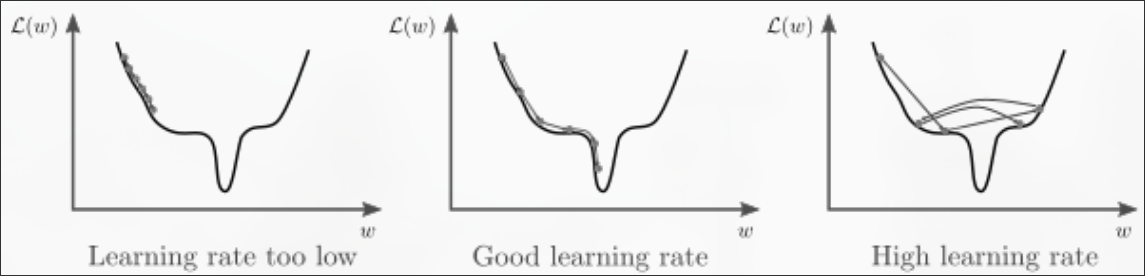
\includegraphics[width=0.7\linewidth]{figures/learning_rate}
\end{figure}

To tune the learning rate, right now is in vogue the \textbf{learning rate decay}, which has formula
\begin{equation*}
  \alpha = \frac{1}{1 + \text{decay\_rate} \cdot \text{current\_epoch}} \cdot \alpha_0
\end{equation*}
Instead a \textbf{not good} learning rate formula is:
\begin{equation*}
  \alpha = e^t \cdot \alpha_0
\end{equation*}

\newpage

\section{Local Optima in Neural Networks}

In a high-dimensional space often, instead of having a shape with a local point like in figure A, we have space that is more like B, which is not so convenient to manage because it's more difficult to find a real local minimum like in A.

\begin{figure}[h]
  \centering
  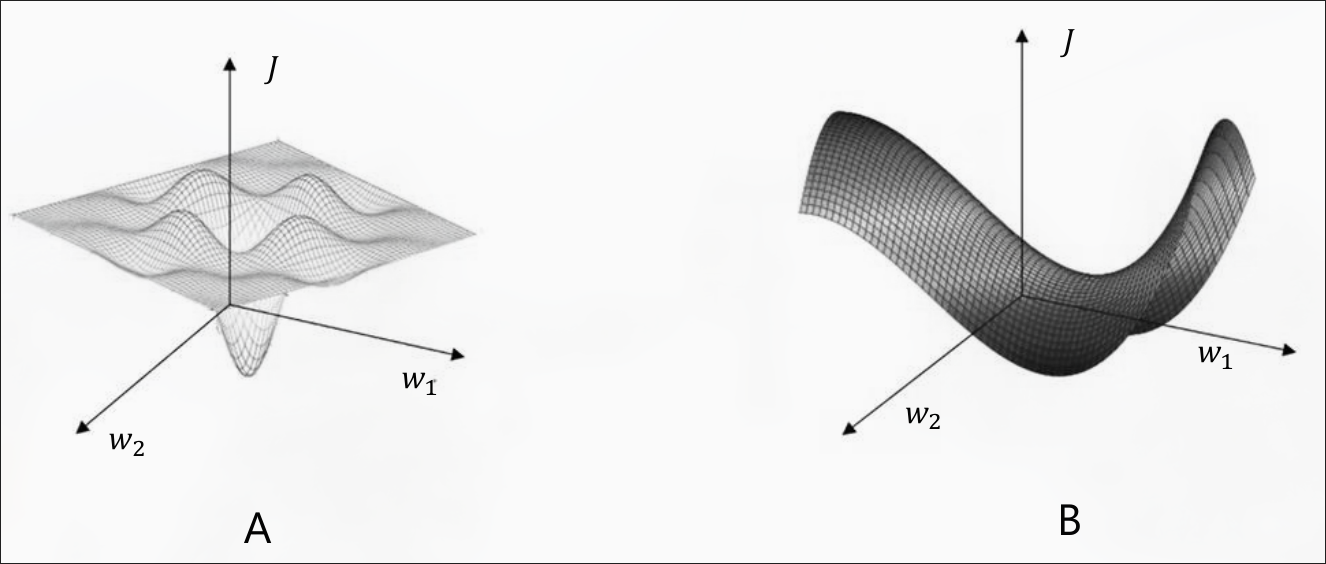
\includegraphics[width=0.75\linewidth]{figures/local_optima}
\end{figure}

In a scenario like figure B the algorithms that we've seen before work better than the plain Gradient Descent.

\chapter{Loss functions}

We've just seen in the chapters before the \textbf{Binary Cross-Entropy Loss}, used for Binary Classification and the \textbf{Mean Squared Error Loss}, used in Regression.

\section{Softmax Activation Layer}

In multi-class classification, the last layer of a neural network is often a Softmax layer, and it means that the network will output a probability distribution over the classes.
Its formula is:
\begin{equation*}
  a^{[i]} = \frac{e^{z^{[i]}}}{\sum_{j=1}^{n} e^{z_j^{[i]}}}
\end{equation*}
where $n$ is the number of classes and $z^{[i]} = W^{[i]} \cdot a^{[i-1]} + b^{[i]}$.
\\\\
Again, this loss function is used for \textbf{multi-class classification}.

\section{Cross-Entropy Loss}

Is the non-binary version, commonly used to quantify the difference between two probability distributions in multi-class classification, and its formula is:
\begin{equation*}
  L(W,b) = - \sum_{i=1}^{m} y^{(i)} \cdot \log \left( h_{W,b} \left( x^{(i)} \right) \right)
\end{equation*}
where $m$ is the number of training samples, $y^{(i)}$ is the ground truth output distribution and $h_{W,b} \left( x^{(i)} \right)$ is the predicted output distribution.

The Cross-Entropy Loss focuses on the \textbf{positive class}, because the negative classes are potentially infinite.

\section{Ranking Loss Function}

Unlike other loss functions, such as Cross-Entropy Loss or Mean Square Error Loss, whose objective is to learn to predict directly a label, a value or a set of values given in input, the objective of Ranking Loss is to predict \textbf{relative distances} between inputs. This task if often called \textbf{metric learning}.

This function computes a \textbf{similarity score} between data points to be able to classify the data, using for example a binary classification, like ``similar'' and ``dissimilar''.

\section{Pairwise Loss Function}

Is a ranking loss function in which we set an \textbf{anchor} sample, for be able to train our model by comparing the anchor against positive (similar) and negative (dissimilar) samples.
For example, a face detection for a specific person, we use a photo of him as an anchor and other images, maybe with different angles and light condition to train the model to predict that is the same person, while also using negative samples, thus samples of other people that the model should identify as different faces.

In this way, we don't work only on strengthening our model over similarities, but also over dissimilarities.

\end{document}
